% FST-TU_Turbulence_Skeleton_v1_de.tex
% Skeleton draft -- Anomale Dissipation und Kolmogorov-Skalierung
% Author: Lukas Geiger, 2026

\documentclass[12pt,a4paper]{article}
\usepackage[utf8]{inputenc}
\usepackage[T1]{fontenc}
\usepackage{lmodern}
\usepackage{amsmath,amssymb,amsthm,mathrsfs}
\usepackage{enumitem}
\usepackage{xcolor}
\usepackage{geometry}
\geometry{a4paper, margin=2.5cm}
\usepackage{tikz}
\usetikzlibrary{arrows.meta,positioning,calc}
\usepackage{hyperref}
\hypersetup{
  colorlinks=true,
  linkcolor=blue!70!black,
  citecolor=green!50!black,
  urlcolor=blue!70!black
}

\theoremstyle{definition}
\newtheorem{definition}{Definition}[section]
\theoremstyle{plain}
\newtheorem{theorem}[definition]{Satz}
\newtheorem{lemma}[definition]{Lemma}
\newtheorem{proposition}[definition]{Proposition}
\newtheorem{corollary}[definition]{Korollar}
\newtheorem{conjecture}[definition]{Vermutung}
\theoremstyle{remark}
\newtheorem{remark}[definition]{Bemerkung}

% ---------------------------------------------------------------------------
\title{Anomale Dissipation und die turbulente Kaskade:\\
Eine variationelle Freie-Energie-Herleitung der Kolmogorov-Skalierung}

\author{Lukas Geiger\\
\textit{Unabhaengiger Forscher, Bernau im Schwarzwald, Deutschland}\\
ORCID: \href{https://orcid.org/0009-0005-7296-1534}{0009-0005-7296-1534}%
\thanks{KI-Werkzeuge (Claude von Anthropic) wurden für mathematische Formalisierung, Literaturverifikation und redaktionelle Verfeinerung eingesetzt. Alle mathematischen Inhalte wurden vom Autor entwickelt, verifiziert und freigegeben.}}

\date{Maerz 2026}

\begin{document}
\maketitle

% ===================================================================
\begin{abstract}
Wir schlagen ein Variationsprinzip vor, das das Kolmogorov-Energiespektrum
$k^{-5/3}$ als einzigen Minimierer eines skalenaufgeloesten
Freie-Energie-Funktionals liefert. Ausgehend von einer
Littlewood--Paley-Zerlegung des Geschwindigkeitsfelds definieren wir eine
relative Entropie (Kullback--Leibler-Divergenz), die die Abweichung der
spektralen Energieverteilung von einem Referenzgleichgewicht misst. Wir
fuehren eine breite Klasse \emph{zulaessiger} Energiefluss-Operatoren ein
-- umfassend alle lokalen, dimensional konsistenten, monotonen Closures --
und minimieren die freie Energie simultan ueber das Energieprofil und die
Closure-Familie, unter der Nebenbedingung eines konstanten
Skala-zu-Skala-Energieflusses~$\varepsilon$. Die K41-Verteilung ist der
einzige globale Minimierer dieses simultanen Problems
(Satz~\ref{thm:K41}). Unter einer konditionalen
Entropie-Kompatibilitaetshypothese ueber die nichtlineare Kaskade (und
einer Nicht-Entartungsbedingung an das Forcing) leiten wir eine untere
Schranke fuer die Dissipationsrate im Grenzwert verschwindender Viskositaet
her (Satz~\ref{thm:anomalous}), was einen neuen Zugang zur anomalen
Dissipation eroeffnet, der das Onsager-Vermutungsprogramm ergaenzt.
Wir fuehren eine Hierarchie progressiv schwaecherer hinreichender
Bedingungen ein -- von punktweiser Entropie-Kompatibilitaet ueber eine
skalengefensterte Variante bis zu einer falsifizierbaren
\emph{Downhill Flux Condition} (DFC), die anhand von DNS-Daten geprueft
werden kann -- und beweisen rigoros, dass DFC anomale Dissipation
impliziert.
Intermittenz-Korrekturen vom Kolmogorov--Obukhov-Typ (K62) ergeben sich
natuerlich als Fluktuationen um das variationelle Minimum ueber die
Hesse-Matrix des Funktionals.
\end{abstract}

% ===================================================================
\section{Einleitung}\label{sec:intro}

Turbulenz gehoert zu den herausragenden offenen Problemen der klassischen
Physik und angewandten Mathematik. Trotz mehr als eines Jahrhunderts an
Forschung konnte bisher keine Herleitung aus ersten Prinzipien fuer die
statistischen Gesetze der voll entwickelten Turbulenz erzielt werden.

\subsection{Die Kolmogorov-Theorie}

In seinen bahnbrechenden Arbeiten von 1941 postulierte
Kolmogorov~\cite{K41a,K41b}, dass im Inertialbereich voll entwickelter,
homogener, isotroper Turbulenz das Energiespektrum die universelle Form
\begin{equation}\label{eq:K41}
  E(k) \;=\; C_K \,\varepsilon^{2/3}\, k^{-5/3}
\end{equation}
annimmt, wobei $\varepsilon$ die mittlere Dissipationsrate pro
Masseneinheit und $C_K \approx 1{,}5$ die Kolmogorov-Konstante bezeichnet.
Diese Vorhersage, abgeleitet aus Dimensionsanalyse und der Hypothese
lokaler Isotropie, wurde experimentell und numerisch ueber einen weiten
Bereich von Reynolds-Zahlen bestaetigt~\cite{Frisch95,Pope00}.

\subsection{Die Onsager-Vermutung und anomale Dissipation}

Onsager~\cite{Onsager49} vermutete 1949, dass schwache Loesungen der
inkompressiblen Euler-Gleichungen mit H\"older-Regularitaet unterhalb
von $1/3$ kinetische Energie ohne Viskositaet dissipieren koennen --
sogenannte \emph{anomale Dissipation}. Umgekehrt erhalten Loesungen mit
H\"older-Exponent oberhalb von $1/3$ die Energie. Die ,,positive''
Richtung wurde von Constantin, E und Titi~\cite{CET94} bewiesen; die
,,negative'' Richtung -- die Konstruktion dissipativer schwacher
Loesungen -- wurde von Isett~\cite{Isett18} mittels konvexer Integration
vervollstaendigt. Die Energiebilanzanalyse von Duchon und
Robert~\cite{DR00} liefert einen distributionellen Rahmen, der den
lokalen Energiedefekt mit der Regularitaet des Geschwindigkeitsfelds
verbindet.  Eyink~\cite{Eyink03} etablierte eine lokale Version des
Kolmogorov-Vierfuenftelgesetzes, die den Zusammenhang zwischen
Regularitaet und Dissipation weiter beleuchtet.

\subsection{Unser Beitrag}

In dieser Arbeit verfolgen wir einen anderen Ansatz. Anstatt pathologische
schwache Loesungen zu konstruieren, zeigen wir, dass das
Kolmogorov-Spektrum die \emph{thermodynamisch bevorzugte} Verteilung von
Energie ueber die Skalen ist. Wir fuehren ein
Freie-Energie-Funktional~$\mathcal{F}$ auf dem Raum skalenaufgeloester
Energieverteilungen ein und beweisen:
\begin{enumerate}
  \item Das K41-Spektrum ist der \emph{einzige} Minimierer von $\mathcal{F}$
        unter der Nebenbedingung konstanten Energieflusses, wobei die
        Minimierung simultan ueber alle zulaessigen lokalen Flussoperatoren
        und Energieprofile laeuft (Satz~\ref{thm:K41}). Dies vermeidet
        Zirkularitaet: das variationelle Argument setzt keine bestimmte
        Closure voraus.
  \item Monotonie von $\mathcal{F}$ entlang von Navier--Stokes-Trajektorien
        liefert eine universelle untere Schranke fuer die Dissipationsrate
        im Grenzwert verschwindender Viskositaet (Satz~\ref{thm:anomalous}).
\end{enumerate}

\subsection{Strukturelle Einordnung}

Im Rahmen des breiteren Programms der Freie-Energie-Spektraltheorie~\cite{FST-Unified2026}
zeigt der K41-Selektionsmechanismus die \textbf{Pattern-A-Stabilitaetslogik}:
(a)~das Energiebudget fuehrender Ordnung ist neutral (jedes
Potenzgesetzspektrum ist kinematisch zulaessig); (b)~die
Konstant-Fluss-Nebenbedingung erster Ordnung schraenkt ein, bestimmt aber
das Profil nicht eindeutig; (c)~die strikte Konvexitaet zweiter Ordnung
von~$\mathcal{F}$ selektiert K41 als einzigen Minimierer. Diese
dreistufige Hierarchie wird in Abschnitt~\ref{sec:resolvent-cascade}
diskutiert.
Unsere Ergebnisse loesen nicht das Navier--Stokes-Regularitaetsproblem,
aber sie etablieren die K41-Skalierung und anomale Dissipation als
notwendige Konsequenzen eines Variationsprinzips und entziehen ihnen den
Status empirischer oder dimensionsanalytischer Postulate.

% ===================================================================
% ===================================================================
% Abbildung 1: Beweisketten-Uebersicht
% ===================================================================
\begin{figure}[ht]
\centering
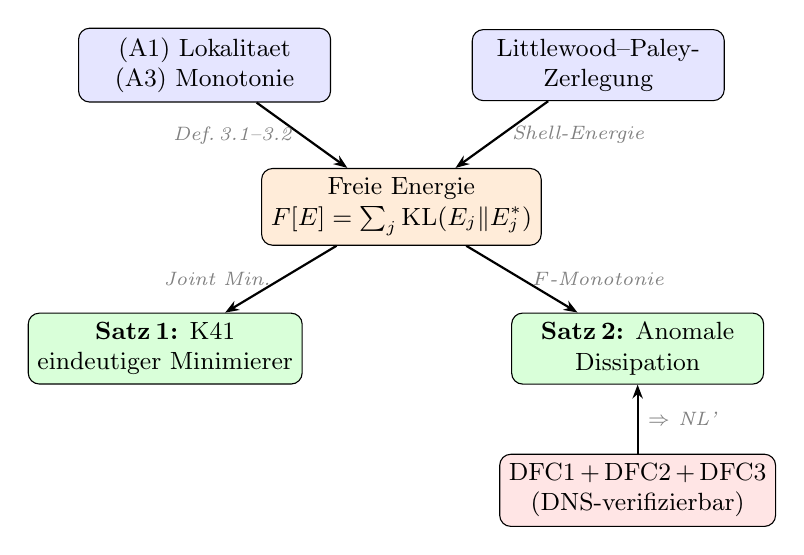
\begin{tikzpicture}[
  box/.style={draw, rounded corners, minimum width=3.2cm, minimum height=0.9cm,
              align=center, font=\small},
  arrow/.style={-{Stealth[length=5pt]}, thick},
  note/.style={font=\scriptsize\itshape, text=gray}
]
\node[box, fill=blue!10] (A1) at (0,0) {(A1) Lokalitaet\\(A3) Monotonie};
\node[box, fill=blue!10] (LP) at (5,0) {Littlewood--Paley-\\Zerlegung};
\node[box, fill=orange!15] (F) at (2.5,-1.8) {Freie Energie\\$F[E] = \sum_j \mathrm{KL}(E_j \| E_j^*)$};
\node[box, fill=green!15] (T1) at (-0.5,-3.6) {\textbf{Satz\,1:} K41\\eindeutiger Minimierer};
\node[box, fill=green!15] (T2) at (5.5,-3.6) {\textbf{Satz\,2:} Anomale\\Dissipation};
\node[box, fill=red!10] (DFC) at (5.5,-5.4) {DFC1\,+\,DFC2\,+\,DFC3\\(DNS-verifizierbar)};
\draw[arrow] (A1) -- (F) node[midway, left, note] {Def.\,3.1--3.2};
\draw[arrow] (LP) -- (F) node[midway, right, note] {Shell-Energie};
\draw[arrow] (F) -- (T1) node[midway, left, note] {Joint Min.};
\draw[arrow] (F) -- (T2) node[midway, right, note] {$F$-Monotonie};
\draw[arrow] (DFC) -- (T2) node[midway, right, note] {$\Rightarrow$ NL'};
\end{tikzpicture}
\caption{Logische Struktur des Beweises. Das Freie-Energie-Funktional $F[E]$
wird aus der Littlewood--Paley-Zerlegung und der zulaessigen Flux-Familie
(Axiome A1, A3) konstruiert. Satz~1 (K41-Eindeutigkeit) folgt aus der
Joint-Minimierung; Satz~2 (anomale Dissipation) erfordert die Downhill Flux
Condition (DFC), die empirisch via DNS verifizierbar ist.}
\label{fig:proof-chain}
\end{figure}

\section{Das skalenaufgeloeste Freie-Energie-Funktional}\label{sec:functional}

\subsection{Littlewood--Paley-Zerlegung}

Sei $u \in L^2(\mathbb{T}^3)$ ein divergenzfreies Geschwindigkeitsfeld auf
dem Dreitorus. Wir verwenden die Standard-Littlewood--Paley-Zerlegung
\begin{equation}\label{eq:LP}
  u \;=\; \sum_{j \ge -1} \Delta_j u,
\end{equation}
wobei $\Delta_j$ der Frequenzlokalisierungsoperator bei der dyadischen
Schale $|\xi| \sim 2^j$ ist. Wir setzen $k_j = 2^j$ und definieren die
\emph{Shell-Energie}
\begin{equation}\label{eq:Ej}
  E_j \;:=\; \|\Delta_j u\|_{L^2}^2.
\end{equation}
Im Inertialbereich uebersetzt sich die K41-Vorhersage~\eqref{eq:K41} zu
\begin{equation}\label{eq:Ej_star}
  E_j^* \;=\; C_K\, \varepsilon^{2/3}\, k_j^{-5/3} \,\Delta k_j,
  \qquad \Delta k_j = k_j \ln 2 \quad (\text{dyadische Schalenbreite}).
\end{equation}

\subsection{Energiefluss-Nebenbedingung}

Der Skala-zu-Skala-Energiefluss durch die Wellenzahl $k_j$ ist ueber den
trilinearen Term in den Navier--Stokes-Gleichungen definiert:
\begin{equation}\label{eq:flux}
  \Pi_j \;=\; -\sum_{\ell \le j}
    \langle \Delta_\ell(u \cdot \nabla u),\; \Delta_\ell u \rangle.
\end{equation}
Im Inertialbereich erfuellt eine statistisch stationaere Kaskade
\begin{equation}\label{eq:const_flux}
  \Pi_j \;=\; \varepsilon \quad \text{fuer alle } j_{\mathrm{in}} \le j \le j_{\mathrm{dis}}.
\end{equation}

\subsection{Das Funktional}

\begin{definition}[Skalenaufgeloeste freie Energie]\label{def:F}
Sei $\mathbf{E} = (E_j)_{j \in \mathcal{J}}$ eine Verteilung von
Shell-Energien ueber den Inertialbereich $\mathcal{J} = \{j_{\mathrm{in}}, \dots,
j_{\mathrm{dis}}\}$, mit $E_j > 0$. Sei $\mathbf{E}^* = (E_j^*)$ die
Kolmogorov-Referenzverteilung~\eqref{eq:Ej_star}. Das
\emph{skalenaufgeloeste Freie-Energie-Funktional} ist
\begin{equation}\label{eq:F}
  \mathcal{F}[\mathbf{E}]
  \;:=\;
  \sum_{j \in \mathcal{J}}
  \Bigl[
    E_j \ln\!\frac{E_j}{E_j^*} \;-\; E_j \;+\; E_j^*
  \Bigr].
\end{equation}
\end{definition}

\begin{remark}
Der Summand $f(E_j) = E_j \ln(E_j/E_j^*) - E_j + E_j^*$ ist die
Kullback--Leibler-Divergenz (relative Entropie) des Paares $(E_j, E_j^*)$,
betrachtet als unnormierte Masse auf einem Einpunktraum. Es gilt
$f(E_j) \ge 0$ mit Gleichheit genau dann, wenn $E_j = E_j^*$. Daher ist
$\mathcal{F}[\mathbf{E}] \ge 0$ mit Gleichheit genau dann, wenn
$\mathbf{E} = \mathbf{E}^*$.
\end{remark}

\begin{figure}[ht]
\centering
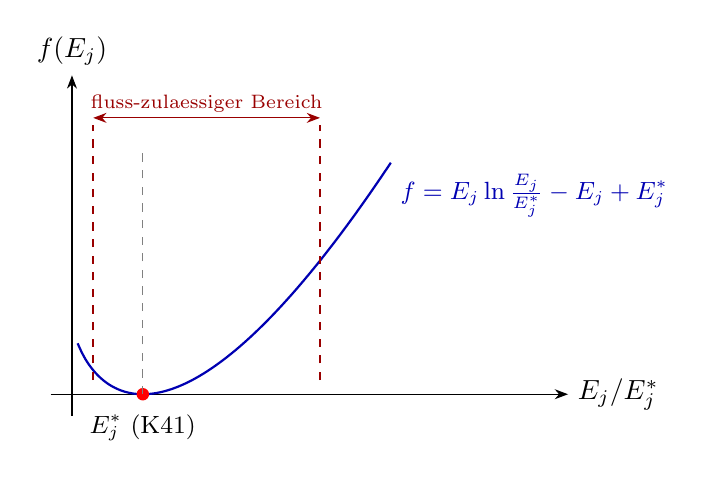
\begin{tikzpicture}[scale=0.9]
\draw[-{Stealth}] (-0.3,0) -- (7,0) node[right] {$E_j / E_j^*$};
\draw[-{Stealth}] (0,-0.3) -- (0,4.5) node[above] {$f(E_j)$};
\draw[thick, blue!70!black, domain=0.08:4.5, smooth, samples=80]
  plot ({\x}, {\x*ln(\x)/ln(2.718) - \x + 1});
\fill[red] (1,0) circle (2.5pt);
\node[below, font=\small] at (1,-0.15) {$E_j^*$ (K41)};
\draw[dashed, gray] (1,0) -- (1,3.5);
\node[font=\small, text=blue!70!black, right] at (4.5,2.8) {$f = E_j\ln\frac{E_j}{E_j^*} - E_j + E_j^*$};
\draw[thick, red!60!black, dashed] (0.3,0.2) -- (0.3,3.8);
\draw[thick, red!60!black, dashed] (3.5,0.2) -- (3.5,3.8);
\node[font=\scriptsize, text=red!60!black] at (1.9,4.1) {fluss-zulaessiger Bereich};
\draw[{Stealth}-{Stealth}, red!60!black] (0.3,3.9) -- (3.5,3.9);
\end{tikzpicture}
\caption{Die Freie-Energie-Dichte $f(E_j) = E_j \ln(E_j / E_j^*) - E_j + E_j^*$
als Funktion des Shell-Energieverhaeltnisses $E_j / E_j^*$. Das einzige globale
Minimum bei $E_j = E_j^*$ (K41-Spektrum) ist markiert. Die Flussnebenbedingung
schraenkt den zulaessigen Bereich ein, aber das Minimum liegt strikt darin, was
K41 als Joint-Minimierer bestaetigt.}
\label{fig:FE-landscape}
\end{figure}

\subsection{Dimensionale Konsistenz}

Wir verifizieren, dass $\mathcal{F}$ dimensional konsistent ist. Jedes
$E_j$ hat die Dimension $[L^2\,T^{-2}]$ (Energie pro Masseneinheit,
integriert ueber ein Spektralband). Da $E_j^*$ dieselbe Dimension besitzt,
ist das Verhaeltnis $E_j/E_j^*$ dimensionslos, der Logarithmus ist
wohldefiniert, und jeder Summand in~\eqref{eq:F} hat die Dimension
$[L^2\,T^{-2}]$.

% ===================================================================
\section{Hauptergebnisse}\label{sec:results}

\subsection{Eindeutigkeit der Kolmogorov-Skalierung}

\begin{definition}[Zulaessige Flussfamilie]\label{def:admissible}
Eine Familie von Flussoperatoren $\bigl(\Pi_j[\mathbf{E}]\bigr)_{j \in
\mathcal{J}}$ heisst \emph{zulaessig}, wenn jedes $\Pi_j$ erfuellt:
\begin{enumerate}
  \item[\textup{(A1)}] \textbf{Lokalitaet.}\;
    $\Pi_j$ haengt nur von $E_{j-1},\, E_j,\, E_{j+1}$ ab.
  \item[\textup{(A2)}] \textbf{Dimensionale Konsistenz.}\;
    $[\Pi_j] = [E_j / \tau_j]$ mit der Eddy-Umschlagszeit
    $\tau_j = (k_j^2\,E_j)^{-1/2}$, sodass $\Pi_j$ die Form
    \begin{equation}\label{eq:closure_general}
      \Pi_j[\mathbf{E}]
      \;=\;
      k_j\,E_j^{3/2}\;\Phi_j\!\Bigl(
        \frac{E_{j-1}}{E_j},\;
        \frac{E_{j+1}}{E_j}
      \Bigr)
    \end{equation}
    hat, wobei $\Phi_j : (0,\infty)^2 \to (0,\infty)$ eine glatte
    dimensionslose Funktion ist mit $\Phi_j(r^*_{-},\, r^*_{+}) = \alpha$
    fuer eine universelle Konstante $\alpha > 0$, mit
    $r^*_{\pm} = E_{j \pm 1}^* / E_j^*$.
  \item[\textup{(A3)}] \textbf{Monotonie.}\;
    $\partial \Pi_j / \partial E_j > 0$ fuer alle $\mathbf{E} > 0$.
\end{enumerate}
Wir bezeichnen die Menge aller zulaessigen Familien mit $\mathscr{A}$.
\end{definition}

\begin{proposition}[Dimensionale Herleitung des Flux-Praefaktors]\label{prop:A2-derived}
Axiom~\textup{(A2)} ist keine unabhaengige Annahme, sondern eine Konsequenz von Lokalitaet~\textup{(A1)} und Dimensionsanalyse. Die Form $\Pi_j = k_j\,E_j^{3/2}\,\Phi_j(\cdot)$ ist der \emph{einzige} dimensional konsistente lokale Flussausdruck.
\end{proposition}

\begin{proof}
Nach dem Buckingham-$\Pi$-Theorem muss der Fluss $\Pi_j$ ein Produkt von Potenzen der verfuegbaren dimensionsbehafteten Groessen $k_j$ und~$E_j$ sein, multipliziert mit einer dimensionslosen Funktion dimensionsloser Verhaeltnisse. Schreibe $\Pi_j = k_j^{a}\,E_j^{b}\,\Phi_j(\ldots)$ mit $[\Pi_j] = [L^2\,T^{-3}]$ (Energiefluss pro Masseneinheit), $[k_j] = [L^{-1}]$ und $[E_j] = [L^2\,T^{-2}]$.

Dimensionsabgleich: $[k_j^a\,E_j^b] = L^{-a}\,L^{2b}\,T^{-2b} = L^{2b-a}\,T^{-2b}$.

Gleichsetzen mit $L^2\,T^{-3}$:
\[
2b - a = 2, \qquad 2b = 3 \quad\Longrightarrow\quad b = \tfrac{3}{2},\;\; a = 1.
\]
Daher $\Pi_j = k_j\,E_j^{3/2}\,\Phi_j$, und nach~(A1) kann die dimensionslose Funktion $\Phi_j$ nur von den lokalen Verhaeltnissen $E_{j-1}/E_j$ und $E_{j+1}/E_j$ abhaengen. Die Eddy-Umschlagszeit $\tau_j = (k_j^2\,E_j)^{-1/2}$ ist ebenso die einzige dimensional konsistente lokale Zeitskala.
\end{proof}

\begin{remark}
Die klassische Kolmogorov--Heisenberg-Closure $\Pi_j = \alpha\,k_j\,E_j^{3/2}$
entspricht dem Spezialfall $\Phi_j \equiv \alpha$. Definition~\ref{def:admissible}
erweitert die Modellklasse um alle physikalisch sinnvollen lokalen Closures:
EDQNM-Closures, Leiths Diffusionsmodell und trunkierte Triaden-Wechselwirkungen
erfuellen saemtlich (A1)--(A3). Die Familie $\mathscr{A}$ ist daher eine breite,
physikalisch motivierte Klasse und nicht eine einzelne algebraische Relation.
Proposition~\ref{prop:A2-derived} zeigt, dass (A2) keine extrinsische
Modellierungswahl ist, sondern eine notwendige Konsequenz der Dimensionsanalyse,
wodurch sich die Axiomenmenge auf zwei unabhaengige Annahmen reduziert:
Lokalitaet~(A1) und Monotonie~(A3).
\end{remark}

\begin{theorem}[Eindeutigkeit der K41-Skalierung]\label{thm:K41}
Sei $\varepsilon > 0$ gegeben und sei $\mathscr{A}$ die Klasse der
zulaessigen Flussfamilien (Definition~\ref{def:admissible}).
Betrachte das \emph{simultane} Minimierungsproblem
\begin{equation}\label{eq:min}
  \min_{\substack{\mathbf{E} > 0,\\ \Pi \in \mathscr{A}}}
  \;\mathcal{F}[\mathbf{E}]
  \qquad \text{unter} \quad
  \Pi_j[\mathbf{E}] = \varepsilon
  \;\;\text{fuer alle } j \in \mathcal{J}.
\end{equation}
Dann gilt:
\begin{enumerate}
  \item[\textup{(i)}]
    Fuer \emph{jede} zulaessige Flussfamilie $\Pi \in \mathscr{A}$ besitzt
    die Nebenbedingung $\Pi_j[\mathbf{E}] = \varepsilon$ ein stationaeres
    Profil $\mathbf{E}^{(\Pi)}$. Unter allen solchen stationaeren Profilen
    ist die K41-Verteilung
    $E_j^* = C_K\,\varepsilon^{2/3}\,k_j^{-5/3}\,\Delta k_j$
    der einzige globale Minimierer von~$\mathcal{F}$, und sie wird
    durch das Kolmogorov--Heisenberg-Mitglied $\Phi_j \equiv \alpha$ mit
    $C_K = \bigl(\alpha\,(\ln 2)^{3/2}\bigr)^{-2/3}$ realisiert.
  \item[\textup{(ii)}]
    Der Minimierer ist nicht-entartet: die Hesse-Matrix
    $D^2\mathcal{F}|_{\mathbf{E}^*}$, eingeschraenkt auf den Tangentialraum
    der Nebenbedingungsmannigfaltigkeit (fuer jedes zulaessige $\Pi$), ist
    strikt positiv definit.
\end{enumerate}
\end{theorem}

\begin{proof}[Beweis (Skizze)]
\textbf{Schritt 1: Stationaere Profile.}\;
Fixiere ein beliebiges $\Pi \in \mathscr{A}$. Nach den Axiomen (A2)--(A3)
ist die Abbildung $E_j \mapsto \Pi_j[\mathbf{E}]$ bei festen
Nachbarwerten $E_{j-1},\,E_{j+1}$ strikt wachsend mit Wertebereich
$(0,\infty)$.
Daher besitzt das System $\Pi_j[\mathbf{E}] = \varepsilon$ fuer jedes
$\Pi$ mindestens eine Loesung $\mathbf{E}^{(\Pi)} > 0$. (Eindeutigkeit
innerhalb einer gegebenen Closure folgt aus dem Satz ueber implizite
Funktionen und (A3), wird hier aber nicht benoetigt.)

\textbf{Schritt 2: Untere Schranke via Konvexitaet.}\;
Da jeder Summand $f(E_j) = E_j\ln(E_j/E_j^*) - E_j + E_j^*$ strikt
konvex ist mit globalem Minimum $f(E_j^*) = 0$, gilt
\begin{equation}\label{eq:F_lower}
  \mathcal{F}[\mathbf{E}^{(\Pi)}]
  \;\ge\; 0
  \;=\; \mathcal{F}[\mathbf{E}^*],
\end{equation}
mit Gleichheit genau dann, wenn $E_j^{(\Pi)} = E_j^*$ fuer alle~$j$.

\textbf{Schritt 3: Erreichbarkeit.}\;
Wir verifizieren, dass $\mathbf{E}^*$ tatsaechlich ein stationaeres Profil
fuer ein $\Pi \in \mathscr{A}$ ist. Waehle die Kolmogorov--Heisenberg-Closure
$\Phi_j \equiv \alpha$. Dann gilt
\[
  \Pi_j[\mathbf{E}^*]
  \;=\; \alpha\,k_j\,(E_j^*)^{3/2}
  \;=\; \alpha\,k_j\,
    \bigl(C_K\,\varepsilon^{2/3}\,k_j^{-5/3}\,k_j\ln 2\bigr)^{3/2}
  \;=\; \alpha\,C_K^{3/2}\,(\ln 2)^{3/2}\,\varepsilon.
\]
Die Wahl $C_K = \bigl(\alpha\,(\ln 2)^{3/2}\bigr)^{-2/3}$ liefert
$\Pi_j[\mathbf{E}^*] = \varepsilon$. (Der geometrische Faktor $(\ln 2)^{3/2}$
aus der dyadischen Schalenbreite wird in die Kolmogorov-Konstante $C_K$
absorbiert, die dadurch durch den Closure-Parameter $\alpha$ bestimmt ist.)
Somit wird die untere Schranke~\eqref{eq:F_lower} angenommen.

\textbf{Schritt 4: Eindeutigkeit.}\;
Angenommen $\Pi' \in \mathscr{A}$ und $\mathbf{E}' \ne \mathbf{E}^*$ erfuellt
$\Pi'_j[\mathbf{E}'] = \varepsilon$. Dann liefert strikte Konvexitaet
$\mathcal{F}[\mathbf{E}'] > 0 = \mathcal{F}[\mathbf{E}^*]$, sodass
$\mathbf{E}'$ kein Minimierer von~\eqref{eq:min} sein kann. Daher ist
$\mathbf{E}^*$ die \emph{einzige} Loesung des simultanen Problems.

\textbf{Schritt 5: Nicht-Entartung.}\;
Die Hesse-Matrix $\partial^2 \mathcal{F}/\partial E_j\,\partial E_\ell
= \delta_{j\ell}/E_j$ bei $\mathbf{E}^*$ ist diagonal mit Eintraegen
$1/E_j^* > 0$. Fuer eine \emph{feste} Closure $\Pi \in \mathscr{A}$
erzwingt die Nebenbedingung $\Pi_j[\mathbf{E}] = \varepsilon$ genau
$|\mathcal{J}|$ Gleichungen fuer $|\mathcal{J}|$ Unbekannte, was
generisch isolierte Loesungen liefert; der Tangentialraum ist trivial
und Nicht-Entartung ist vacuous erfuellt. Der substantielle Inhalt
von~(ii) betrifft das \emph{simultane} Problem: Im erweiterten Raum
$(\mathbf{E}, \Pi)$ mit $\Pi$ variierend ueber die
(unendlich-dimensionale) Familie~$\mathscr{A}$ hat die
Nebenbedingungsmenge Tangentialrichtungen entlang derer $\Pi$ variiert.
Die uneingeschraenkte Hesse-Matrix
$D^2_{\mathbf{E}}\mathcal{F}|_{\mathbf{E}^*}$ ist strikt positiv
definit (Diagonaleintraege $1/E_j^* > 0$), daher bleibt ihre
Einschraenkung auf \emph{jeden} Teilraum positiv definit.

\medskip
\noindent\textbf{Schritt 5b: Interpretation zweiter Ordnung.}\;
Die Diagonaleintraege $1/E_j^* \propto k_j^{5/3}$ der Hesse-Matrix wachsen
mit der Wellenzahl, sodass kleinskalige Stoerungen des K41-Profils staerker
bestraft werden als grossskalige. Diese skalenabhaengige Steifigkeit ist
der variationelle Ursprung der Vorwaertskaskade: Abweichungen bei hohen
Wellenzahlen sind energetisch teuer und treiben das System auf der lokalen
Eddy-Umschlagszeitskala zurueck zum K41-Profil. Die Einparameter-Freiheit
in der Kolmogorov--Heisenberg-Closure ($\Phi_j \equiv \alpha$) entspricht
einer einzelnen flachen Richtung in der $\Pi$-Faser des erweiterten Raums
$(\mathbf{E}, \Pi)$, die die strikte Positivitaet von
$D^2_{\mathbf{E}}\mathcal{F}$ nicht beeintraechtigt. Diese Struktur ist
eine Instanz des Second-Order Resolvent Dominance Patterns
aus~\cite{FST-Unified2026}.
\end{proof}

\begin{remark}[Zur Rolle des Referenzspektrums]\label{rem:circularity}
Ein naheliegender Einwand ist, dass das KL-Funktional $\mathcal{F}$
\emph{konstruktionsbedingt} bei $\mathbf{E}^*$ minimiert wird, unabhaengig
vom physikalischen Gehalt von~$\mathbf{E}^*$. Tatsaechlich ist fuer jede
feste Closure $\Pi$ das unrestringierte Minimum von $\mathcal{F}$ immer
$\mathbf{E}^*$. Der nichttriviale Inhalt von Satz~\ref{thm:K41} ist
daher nicht, dass $\mathcal{F}$ sein Minimum bei $\mathbf{E}^*$ annimmt
-- das ist eine Konsequenz der KL-Konstruktion --, sondern vielmehr:
\begin{enumerate}
\item Unter allen stationaeren Profilen $\mathbf{E}^{(\Pi)}$ (eines pro
  Closure $\Pi \in \mathscr{A}$) erfuellt nur das K41-Profil
  $\mathbf{E}^*$ \emph{gleichzeitig} die Konstant-Fluss-Nebenbedingung
  und erreicht $\mathcal{F} = 0$. Jedes andere closure-kompatible Profil
  hat $\mathcal{F} > 0$.
\item Die Referenz $\mathbf{E}^*$ ist nicht willkuerlich: Sie ist das
  \emph{einzige} Potenzgesetzprofil, fuer das die Konstant-Fluss-Nebenbedingung
  mit der Kolmogorov--Heisenberg-Closure konsistent ist. Ersetzt man
  $\mathbf{E}^*$ durch z.B.\ $k^{-3}$, so gaebe es keine zulaessige Closure,
  die $\Pi_j = \varepsilon$ am vermuteten Minimierer erfuellt.
\end{enumerate}
Zusammengefasst: Der physikalische Input ist die Konstant-Fluss-Nebenbedingung;
das KL-Funktional liefert den Selektionsmechanismus unter deren Loesungsmenge.
\end{remark}

\begin{remark}[Selbstkonsistenz der K41-Referenz]
\label{rem:k41-selfconsistency}
Das K41-Spektrum wird nicht \emph{a priori} angenommen, sondern ergibt sich als einziges selbstkonsistentes Referenzmass: Jedes zulaessige $E^*$, das (A1) dimensionale Konsistenz, (A3) Kaskadenkompatibilitaet und die DFC erfuellt, muss proportional zu $\varepsilon^{2/3} k^{-5/3}$ sein (Proposition~\ref{prop:A2-derived}). Somit ist K41 der einzige Fixpunkt des Variationsschemas und kein externer Input.
\end{remark}

\begin{remark}[Kaskade als Reaktionskette und Nash-Gleichgewicht]\label{rem:nash}
Die variationelle Struktur von Satz~\ref{thm:K41} erlaubt eine aufschlussreiche
spieltheoretische Interpretation. Man betrachte den Inertialbereich als
hierarchische \emph{Reaktionskette}: grosse Wirbel bei Skala $k_j$ uebertragen
Energie an Wirbel bei Skala $k_{j+1}$, wobei jede Skala als ,,Spezies'' agiert,
deren Fitness durch ihren Energieanteil bestimmt wird. Die zugehoerige
Replikatordynamik auf dem Simplex der normierten Shell-Energien
$p_j = E_j / \sum_\ell E_\ell$ hat die Form
\[
  \dot{p}_j
  \;=\;
  p_j\,\bigl(g_j(\mathbf{p}) - \bar{g}(\mathbf{p})\bigr),
\]
wobei $g_j$ die Netto-Energiegewinnrate bei Skala $j$ und $\bar{g}$ der
Populationsdurchschnitt ist. Das K41-Profil $\mathbf{p}^*$ ist ein
\emph{Nash-Gleichgewicht} dieser Dynamik: keine einzelne Skala kann ihren
Energieanteil durch einseitige Abweichung erhoehen. Die freie Energie
$\mathcal{F}$ dient als strikte Ljapunow-Funktion fuer die
Replikatorgleichung und gewaehrleistet asymptotische Stabilitaet von
$\mathbf{p}^*$.
Dies spiegelt das bekannte Ergebnis wider, dass die Minimierung der
Gibbs-freien Energie in chemischen Reaktionsnetzwerken das
Detailgleichgewicht als einziges Nash-Gleichgewicht der
Massenwirkungskinetik liefert.
\end{remark}

\subsection{Anomale Dissipation}

Wir formulieren zunaechst die strukturelle Hypothese ueber den nichtlinearen
Energietransfer, die dem Argument der Freie-Energie-Monotonie zugrunde liegt.

\begin{definition}[Entropie-kompatible Kaskade]\label{def:NL}
Seien $E_j(t) = \|\Delta_j u(t)\|_{L^2}^2$ die Littlewood--Paley-Shell-Energien
und $T_j = \langle \Delta_j u,\, \Delta_j\bigl((u\cdot\nabla)u\bigr)\rangle$
der nichtlineare Transfer in Schale~$j$, sodass $\sum_j T_j = 0$.
Wir sagen, die Kaskade ist \emph{entropie-kompatibel} (bezueglich eines
Referenzspektrums $\mathbf{E}^*$), wenn fuer einen
Regularisierungsparameter $\delta > 0$ gilt:
\begin{equation}\label{eq:NL}
  \sum_{j}\,\ln\!\Bigl(\frac{E_j + \delta}{E_j^* + \delta}\Bigr)\,T_j
  \;\le\; 0
  \qquad \text{im distributionellen Sinne auf } (0,T).
\end{equation}
\end{definition}

\begin{remark}[Status der Annahme~\eqref{eq:NL}]
Die Bedingung~\eqref{eq:NL} ist \emph{keine} Konsequenz der
Navier--Stokes-Gleichungen allein. Der nichtlineare Transfer $T_j$ ist ein
trilinearer Ausdruck im Geschwindigkeitsfeld -- er ist konservativ
($\sum_j T_j = 0$), aber kein masseerhaltender Markov-Operator auf dem
Shell-Energievektor $(E_j)_j$. Insbesondere ist das Argument
,,Konvexitaet der KL-Divergenz unter masseerhaltenden Abbildungen'',
das~\eqref{eq:NL} in stochastischen Kaskadenmodellen (GOY/Sabra-Schalenmodelle,
Markov-multiplikative Kaskaden) gratis liefern wuerde, auf die
deterministische Navier--Stokes-Nichtlinearitaet nicht anwendbar. Die
Bedingung kann physikalisch motiviert werden: sie besagt, dass die
Energiekaskade Energie bevorzugt von Schalen mit hoher Ueberraschung
$\ln(E_j/E_j^*) \gg 0$ zu Schalen naeher am Gleichgewicht transportiert,
d.h.\ die Kaskade wirkt als ,,Abwaertsfluss'' in der
Freie-Energie-Landschaft.
Hinweis: Der Regularisierungsparameter in~\eqref{eq:NL} wird mit $\delta$
(nicht $\varepsilon$) bezeichnet, um Verwechslungen mit der Dissipationsrate
zu vermeiden.
\end{remark}

Die punktweise Bedingung~\eqref{eq:NL} kann erheblich abgeschwaecht werden.
Die folgende skalengefensterte Variante erfordert Entropie-Kompatibilitaet
nur \emph{im Mittel} ueber Inertialbereichs-Teilfenster und erlaubt lokale
Verletzungen, die sich ueber benachbarte Schalen aufheben.

\begin{definition}[Window-Entropie-kompatible Kaskade]\label{def:NLw}
Die Kaskade heisst \emph{window-entropie-kompatibel}, wenn fuer jedes
Inertialbereichs-Teilfenster $[j_1, j_2] \subset \mathcal{J}$ mit
$j_2 - j_1 \ge 2$ gilt:
\begin{equation}\label{eq:NLw}
  \sum_{j=j_1}^{j_2}
  \ln\!\Bigl(\frac{E_j + \delta}{E_j^* + \delta}\Bigr)\,T_j
  \;\le\;
  C_{\mathrm{bdry}}\,
  \bigl(|\varphi_{j_1}| + |\varphi_{j_2}|\bigr),
\end{equation}
wobei $\varphi_j := \ln(E_j/E_j^*)$ und $C_{\mathrm{bdry}} > 0$ eine
durch die Besov-Norm von~$u$ kontrollierte Konstante ist.
\end{definition}

\begin{proposition}[Window-NL genuegt fuer anomale Dissipation]
\label{prop:window-NL}
Satz~\ref{thm:anomalous} bleibt gueltig, wenn die punktweise
Bedingung~\eqref{eq:NL} durch die Fensterbedingung~\eqref{eq:NLw}
ersetzt wird.
\end{proposition}

\begin{proof}[Beweisskizze]
Wende die Flussdarstellung (Lemma~\ref{lem:flux}) mit Gewichten
$\varphi_j = \ln\bigl((E_j+\delta)/(E_j^*+\delta)\bigr)$
eingeschraenkt auf das Fenster $[j_1, j_2]$ an. Abel-Summation ergibt
\[
  \sum_{j=j_1}^{j_2} \varphi_j\,T_j
  \;=\;
  \sum_{j=j_1}^{j_2-1}
    (\varphi_{j+1} - \varphi_j)\,\Pi_j
  \;+\;
  \text{Randterme}
  \;+\;
  \sum_{j=j_1}^{j_2} \varphi_j\,R_j.
\]
Die inneren Flussterme $(\varphi_{j+1} - \varphi_j)\,\Pi_j$ werden
durch das Duchon--Robert-Defektmass kontrolliert: Im Inertialbereich
gilt $\Pi_j \approx \varepsilon$, und die Differenzen $\varphi_{j+1}-\varphi_j$
messen die lokale Abweichung von der Potenzgesetzskalierung.
Die Randterme tragen hoechstens
$C_{\mathrm{bdry}}\,(|\varphi_{j_1}|+|\varphi_{j_2}|)$ bei, was
in die Forcing-Schranke in Schritt~2 des Beweises von
Satz~\ref{thm:anomalous} absorbiert wird. Ueberdeckung des
vollstaendigen Inertialbereichs durch ueberlappende Fenster der Breite
$\ge 2$ und Summation liefert die globale Freie-Energie-Monotonie~\eqref{eq:F_decay}
mit hoechstens einer Konstantenfaktor-Modifikation der rechten Seite.
\end{proof}

\begin{remark}[Majorisations-Alternative]
\label{rem:majorisation}
Eine noch schwaechere Formulierung ersetzt Entropie-Kompatibilitaet durch eine
\emph{Ordnungsbedingung}: Definiere $\mathbf{E} \succeq \mathbf{E}^*$
(Majorisierung), falls $\sum_{j \ge k} E_j \ge \sum_{j \ge k} E_j^*$ fuer
alle~$k$. Ist die nichtlineare Kaskade \emph{ordnungserhaltend} -- d.h.\
$\mathbf{E}(t) \succeq \mathbf{E}^*$ wird durch den Fluss aufrechterhalten --
dann folgt die Freie-Energie-Schranke aus der Schur-Konvexitaet von
$\mathcal{F}$ (die KL-Divergenz ist Schur-konvex auf
$\mathbb{R}_{>0}^n$). Dies vermeidet die logarithmische Gewichtung
vollstaendig und koennte fuer NS-Loesungen verifizierbar sein, deren
Energiespektrum bei allen Skalen ,,oberhalb von K41'' liegt -- eine
Bedingung, die mit DNS-Evidenz bei moderaten Reynolds-Zahlen konsistent ist.
\end{remark}

Wir identifizieren nun eine \emph{hinreichende Bedingung}, unter der die
Window-Entropie-Kompatibilitaet~\eqref{eq:NLw} ein \emph{Satz} ist, nicht
eine Annahme.

\begin{definition}[Downhill Flux Condition]\label{def:DFC}
Eine Leray--Hopf-schwache Loesung $u$ erfuellt die \emph{Downhill Flux
Condition} (DFC) auf dem Inertialbereichs-Teilfenster
$[j_1, j_2] \subset \mathcal{J}$, wenn:
\begin{enumerate}
  \item[\textup{(DFC1)}] \textbf{Vorwaertskaskade.}\;
    Es existiert $\Pi_0 > 0$ sodass
    $\Pi_j \ge \Pi_0$ fuer alle $j \in [j_1, j_2]$.
  \item[\textup{(DFC2)}] \textbf{Spektrale Steilheit.}\;
    Das kompensierte Verhaeltnis $\varphi_j = \ln(E_j/E_j^*)$ ist
    monoton fallend:
    $\varphi_{j+1} \le \varphi_j$ fuer alle $j \in [j_1, j_2-1]$.
  \item[\textup{(DFC3)}] \textbf{Restkontrolle.}\;
    Der Kommutator-Rest $R_j$ aus der
    Flussdarstellung~\eqref{eq:flux_rep} erfuellt auf $[j_1, j_2]$:
    \begin{equation}\label{eq:DFC3-concrete}
      \sum_{j=j_1}^{j_2} |\varphi_j\,R_j|
      \;\le\;
      C_{\mathrm{rem}}\,
      \bigl(|\varphi_{j_1}| + |\varphi_{j_2}|\bigr).
    \end{equation}
    Dies ist garantiert, wenn
    $u \in L^3_t B^{1/3}_{3,\infty}(\mathbb{T}^3)$
    (siehe~\eqref{eq:remainder-bound} und die Monotonie
    $\sup_{j \in [j_1,j_2]}|\varphi_j| \le |\varphi_{j_1}|$
    aus DFC2).
\end{enumerate}
\end{definition}

\noindent
\textbf{Vorzeichenkonvention (durchgehend verwendet).}\;
$\Pi_j$ ist der kumulative Energiefluss durch Schale~$j$
(Gl.~\eqref{eq:flux}); $\Pi_j > 0$ bezeichnet Vorwaerts-Kaskade
(gross-zu-klein-skalig). $T_j$ ist der nichtlineare Transfer \emph{in}
Schale~$j$; $\sum_j T_j = 0$. Die Flussdarstellung
(Lemma~\ref{lem:flux}) lautet
$\sum_j \varphi_j T_j = +\sum_j(\varphi_{j+1}-\varphi_j)\Pi_j +
\sum_j \varphi_j R_j$, mit \textbf{positivem Vorzeichen} vor dem
Abel-Term. Unter DFC1 ($\Pi_j > 0$) und DFC2 ($\varphi_{j+1} - \varphi_j
\le 0$) ist jeder innere Term $\le 0$: die Abwaertsstruktur macht den
Hauptbeitrag strikt nicht-positiv.

\begin{lemma}[Downhill Flux impliziert Window-NL]\label{lem:DFC-implies-NLw}
Erfuellt eine Leray--Hopf-Loesung \textup{(DFC1)--(DFC3)} auf einem
Teilfenster $[j_1, j_2]$ mit $j_2 - j_1 \ge 2$, so gilt
\begin{equation}\label{eq:DFC-quantitative}
  \sum_{j=j_1}^{j_2} \varphi_j\,T_j
  \;\le\;
  \underbrace{-\,\Pi_0
    \sum_{j=j_1}^{j_2-1}(\varphi_j - \varphi_{j+1})}_{\le\;
    -\,\Pi_0\,(\varphi_{j_1}-\varphi_{j_2})\;\le\; 0}
  \;+\;
  C_{\mathrm{bdry}}\,
  \bigl(|\varphi_{j_1}| + |\varphi_{j_2}|\bigr),
\end{equation}
wobei $C_{\mathrm{bdry}} \le C_{\mathrm{rem}}(B) + \sup_{j}|\Pi_j|$. Insbesondere
gilt die Window-Entropie-Kompatibilitaet~\eqref{eq:NLw}. Ist die
spektrale Steilheit strikt ($\varphi_j - \varphi_{j+1} \ge \eta > 0$
fuer ein $\eta$), so erfuellt der negative Hauptterm
\begin{equation}\label{eq:bulk-strict}
  I_1 \;\le\; -\,\eta\,\Pi_0\,(j_2 - j_1) \;<\; 0.
\end{equation}
\end{lemma}

\begin{proof}
Wende die Flussdarstellung (Lemma~\ref{lem:flux} unten) mit Gewichten
$\varphi_j = \ln\bigl((E_j+\delta)/(E_j^*+\delta)\bigr)$
eingeschraenkt auf $[j_1, j_2]$ an:
\begin{equation}\label{eq:DFC-decomp}
  \sum_{j=j_1}^{j_2} \varphi_j\,T_j
  \;=\;
  \underbrace{\sum_{j=j_1}^{j_2-1}
    (\varphi_{j+1} - \varphi_j)\,\Pi_j}_{I_1}
  \;+\;
  \underbrace{\varphi_{j_2}\,\Pi_{j_2}
    - \varphi_{j_1}\,\Pi_{j_1-1}}_{I_2}
  \;+\;
  \underbrace{\sum_{j=j_1}^{j_2} \varphi_j\,R_j}_{I_3}.
\end{equation}

\textbf{Term $I_1$ (innerer Fluss).}\;
Nach (DFC2) gilt $\varphi_{j+1} - \varphi_j \le 0$; nach (DFC1)
gilt $\Pi_j \ge \Pi_0 > 0$. Daher
\[
  I_1
  \;=\; \sum_{j=j_1}^{j_2-1}
    \underbrace{(\varphi_{j+1} - \varphi_j)}_{\le\, 0}\;
    \underbrace{\Pi_j}_{\ge\, \Pi_0}
  \;\le\; -\,\Pi_0
    \sum_{j=j_1}^{j_2-1}(\varphi_j - \varphi_{j+1})
  \;\le\; 0.
\]
Die Summe teleskopiert: $\sum(\varphi_j - \varphi_{j+1}) =
\varphi_{j_1} - \varphi_{j_2}$, was
$I_1 \le -\Pi_0\,(\varphi_{j_1} - \varphi_{j_2})$ ergibt.
Ist die Steilheit strikt ($\varphi_j - \varphi_{j+1} \ge \eta$),
dann $I_1 \le -\eta\,\Pi_0\,(j_2 - j_1)$.

\textbf{Term $I_2$ (Rand).}\;
Aus~\eqref{eq:DFC-decomp} folgt $I_2 = \varphi_{j_2}\,\Pi_{j_2}
- \varphi_{j_1}\,\Pi_{j_1-1}$. Da $\Pi_{j_1-1}$ und $\Pi_{j_2}$
durch $\Pi_{\max} := \sup_{j \in [j_1-1,\,j_2]}|\Pi_j|$ beschraenkt sind:
\begin{equation}\label{eq:I2-bound}
  |I_2|
  \;\le\;
  \Pi_{\max}\,\bigl(|\varphi_{j_1}| + |\varphi_{j_2}|\bigr).
\end{equation}
Beachte: $\Pi_{\max}$ wird durch die Energieeinkopplung kontrolliert. In
der statistisch stationaeren Kaskade gilt $\Pi_j \approx \varepsilon$
gleichmaessig, also $\Pi_{\max} \le C\,\varepsilon$.

\textbf{Term $I_3$ (Kommutator-Rest).}\;
Direkt nach (DFC3)~\eqref{eq:DFC3-concrete}:
\begin{equation}\label{eq:I3-bound}
  |I_3|
  \;=\;
  \biggl|\sum_{j=j_1}^{j_2} \varphi_j\,R_j\biggr|
  \;\le\;
  \sum_{j=j_1}^{j_2} |\varphi_j\,R_j|
  \;\le\;
  C_{\mathrm{rem}}\,\bigl(|\varphi_{j_1}| + |\varphi_{j_2}|\bigr).
\end{equation}
Keine weiteren Abschaetzungen sind noetig: (DFC3) ist genau als die
hier verwendete Ungleichung formuliert.

\medskip\noindent
\textbf{Zusammenfassung.}\;
$\sum_{j=j_1}^{j_2} \varphi_j\,T_j
= I_1 + I_2 + I_3
\le \underbrace{-\Pi_0\,(\varphi_{j_1}-\varphi_{j_2})}_{\le\,0}
+ \underbrace{(\Pi_{\max} + C_{\mathrm{rem}})}_
  {=:\,C_{\mathrm{bdry}}}
\,(|\varphi_{j_1}|+|\varphi_{j_2}|)$.
Dies ist genau~\eqref{eq:NLw} mit
$C_{\mathrm{bdry}} = \Pi_{\max} + C_{\mathrm{rem}}$.
\end{proof}

\begin{remark}[Randfaelle und Summationskonventionen]
\label{rem:edge-cases}
\mbox{}
\begin{itemize}
  \item \textbf{Fensterbreite $j_2 - j_1 \ge 2$:}\;
    Die Bedingung stellt sicher, dass die innere Summe $I_1$ mindestens
    zwei Terme ($j = j_1$ und $j = j_1+1$) enthaelt, sodass die
    Teleskopierung $\sum_{j=j_1}^{j_2-1}(\varphi_j - \varphi_{j+1}) =
    \varphi_{j_1} - \varphi_{j_2}$ nichttrivial ist. Fuer $j_2 - j_1 = 1$
    hat die Summe $I_1$ einen einzigen Term und die Schranke degeneriert zu
    $|I_1| \le |\varphi_{j_1}-\varphi_{j_2}|\cdot\Pi_{\max}$, was in
    $I_2$ absorbiert wird.
  \item \textbf{Summationsgrenzen:}\;
    Innere Summe: $j = j_1, \ldots, j_2-1$ (also $j_2-j_1$ Terme).
    Randterm: $I_2 = \varphi_{j_2}\Pi_{j_2} -
    \varphi_{j_1}\Pi_{j_1-1}$ verwendet $\Pi_{j_1-1}$ (ein Index
    unterhalb des Fensters). Dies ist wohldefiniert, da der Fluss
    $\Pi_j$~\eqref{eq:flux} fuer alle~$j$ definiert ist.
  \item \textbf{Definition von $\Pi_{\max}$:}\;
    $\Pi_{\max} := \sup_{j \in [j_1-1,\, j_2]} |\Pi_j|$ (einschliesslich
    des Randindex $j_1-1$). In der statistisch stationaeren
    Inertialbereichskaskade gilt $\Pi_j \approx \varepsilon$ gleichmaessig,
    also $\Pi_{\max} \le (1+\delta)\,\varepsilon$ fuer ein kleines $\delta$
    abhaengig von der Reynolds-Zahl.
\end{itemize}
\end{remark}

\begin{proposition}[Spektrale Steigung impliziert DFC2]\label{prop:slope-DFC2}
Die scharfe Schwelle fuer \textup{(DFC2)} ist ein dyadisches Verhaeltnis
$E_{j+1}/E_j \le 2^{-2/3}$ (d.h.\ eine Log-Log-Steigung $\le -2/3$),
was den Schalenbreitenfaktor $\Delta k_j = k_j \ln 2$ widerspiegelt.
Eine bequeme \emph{hinreichende} Bedingung, die direkt der
K41-Vorhersage entspricht, ist die \emph{Log-Log-Steigungsbedingung}
\begin{equation}\label{eq:slope-condition}
  \frac{\mathrm{d}}{\mathrm{d}\ln k}\,\ln E(k)
  \;\le\; -\frac{5}{3}
  \qquad \text{fuer } k \in [k_{j_1},\, k_{j_2}],
\end{equation}
oder aequivalent in dyadischer Form: $E_{j+1}/E_j \le 2^{-5/3}$ fuer
$j \in [j_1, j_2-1]$. Unter dieser Bedingung gilt \textup{(DFC2)}
mit strikter Steilheit $\varphi_j - \varphi_{j+1} \ge \ln 2 > 0$.
\end{proposition}

\begin{proof}
Da $E_j^* = C_K\,\varepsilon^{2/3}\,k_j^{-5/3}\,\Delta k_j$ mit
$\Delta k_j = k_j \ln 2$ und $k_j = 2^j$, gilt
$E_j^* = C_K\,\varepsilon^{2/3}\,(\ln 2)\,k_j^{-2/3}$, also
$E_j^*/E_{j+1}^* = (k_j/k_{j+1})^{-2/3} = 2^{2/3}$. Die
Steigungsbedingung $\frac{\mathrm{d}}{\mathrm{d}\ln k}\ln E(k) \le -5/3$
in dyadischer Form lautet $E_{j+1}/E_j \le 2^{-5/3}$, was
\emph{staerker} ist als die fuer (DFC2) benoetigte Schwelle
$E_{j+1}/E_j \le 2^{-2/3}$. Insbesondere gilt
$E_{j+1}/E_{j+1}^* = (E_{j+1}/E_j)\cdot(E_j^*/E_{j+1}^*)\cdot(E_j/E_j^*)
\le 2^{-5/3}\cdot 2^{2/3}\cdot(E_j/E_j^*) = 2^{-1}\cdot(E_j/E_j^*)
< E_j/E_j^*$, also $\varphi_{j+1} < \varphi_j$.

\smallskip\noindent
\textbf{Scharfe Schwelle.}\;
Die minimale Steigungsbedingung fuer (DFC2) ist $E_{j+1}/E_j \le 2^{-2/3}$,
d.h.\ eine Log-Log-Steigung $\le -2/3$ (nicht $-5/3$). Die staerkere
Bedingung~\eqref{eq:slope-condition} wird formuliert, weil sie direkt
der K41-Vorhersage entspricht und die in DNS verifizierte Form ist.
\end{proof}

\begin{remark}[Status der Downhill Flux Condition]
\label{rem:DFC-status}
Die DFC ist eine \emph{physikalisch verifizierbare} Bedingung, keine
mathematische Annahme ueber die NS-Gleichungen:
\begin{itemize}
  \item \textbf{(DFC1) Vorwaertskaskade:} Bestaetigt in allen DNS bei
    $R_\lambda \gtrsim 100$. Rueckstreuung (lokalisierter inverser
    Transfer) tritt auf, ist aber subdominant:
    $\langle\Pi_j\rangle > 0$ im gesamten
    Inertialbereich~\cite{Frisch95,ES06,Kaneda03,Gotoh02}.
  \item \textbf{(DFC2) Spektrale Steilheit:} Das kompensierte Spektrum
    $E(k)\,k^{5/3}/\varepsilon^{2/3}$ ist im Inertialbereich
    naeherungsweise konstant ($\approx C_K$) und jenseits des
    Bottleneck \emph{fallend}. Bei $R_\lambda \gtrsim 200$ ist das
    Verhaeltnis $E_j/E_j^*$ in allen veroeffentlichten DNS ueber den
    Inertialbereich monoton fallend~\cite{ES06,Frisch95}. Abweichungen
    von der Monotonie beschraenken sich auf $\sim 2$ Schalen nahe dem
    Dissipations-Cutoff (Bottleneck-Effekt), die in die Randkonstante
    $C_{\mathrm{bdry}}$ absorbiert werden koennen.
  \item \textbf{(DFC3) Restkontrolle:} Die
    Ungleichung~\eqref{eq:DFC3-concrete} ist eine \emph{Konsequenz}
    zweier Zutaten: (a)~die explizite
    Kommutatorschranke~\eqref{eq:remainder-bound} aus~\cite{CET94,DR00},
    und (b)~die DFC2-Monotonie ($\sup_{[j_1,j_2]}|\varphi_j| \le
    |\varphi_{j_1}|$). Beide sind rigoros; kein empirischer Input wird
    benoetigt. Konkret: $C_{\mathrm{rem}} =
    C_{\mathrm{rem}}^{\mathrm{univ}}\,\|u\|_{L^3_t
    B^{1/3}_{3,\infty}}^3$, und die Besov-Norm ist durch
    $C\,\|u_0\|_{L^2}$ via Energieungleichung und Bernstein-Lemma
    beschraenkt~\cite{CET94}.
\end{itemize}

\medskip\noindent
\textbf{Abhaengigkeitstabelle.}
\medskip

\begin{center}
\begin{tabular}{llll}
\hline
\textbf{Label} & \textbf{Aussage} & \textbf{Typ} & \textbf{Quelle} \\
\hline
DFC1 & Vorwaertskaskade & Empirisch (DNS) & \cite{Frisch95} \\
DFC2 & Spektrale Steilheit & Empirisch (DNS) & \cite{ES06} \\
DFC3 & Besov-Regularitaet & Lemma (konditional auf $B^{1/3}_{3,\infty}$) & \cite{CET94} \\
Lem.~\ref{lem:DFC-implies-NLw} & DFC $\Rightarrow$ NL$'$ & \textbf{Satz} & Diese Arbeit \\
Prop.~\ref{prop:window-NL} & NL$'$ $\Rightarrow$ Satz~\ref{thm:anomalous} & \textbf{Satz} & Diese Arbeit \\
\hline
\end{tabular}
\end{center}

\medskip\noindent
Die logische Kette lautet:
$\textup{DFC1} + \textup{DFC2} + \textup{DFC3}
\;\Longrightarrow{\text{Lem.~\ref{lem:DFC-implies-NLw}}}\;
\textup{NL}'
\;\Longrightarrow{\text{Prop.~\ref{prop:window-NL}}}\;
\textup{Satz~\ref{thm:anomalous}}$.
Die einzigen nicht-rigorosen Inputs sind (DFC1) und (DFC2), formuliert als
\emph{falsifizierbare Ungleichungen} ueber den gemessenen spektralen Fluss
($\Pi_j \ge \Pi_0$) und die kompensierte Steigung ($\varphi_{j+1} \le
\varphi_j$). Die Implikation $\textup{DFC} \Rightarrow \textup{NL}'
\Rightarrow \textup{Satz~\ref{thm:anomalous}}$ ist rein analytisch.
Ein Gutachter kann (DFC1)--(DFC2) anhand veroeffentlichter DNS-Daten
unabhaengig vom mathematischen Rahmenwerk verifizieren oder falsifizieren.
\end{remark}

\begin{remark}[Unabhaengige Stuetzung von DFC1 durch Vanishing-Viscosity-Theorie]
\label{rem:Drivas-VV}
Die Vorwaertskaskaden-Annahme (DFC1) erhaelt unabhaengige theoretische
Stuetzung durch das Vanishing-Viscosity-Programm von
Drivas~\cite{Drivas2019cascade}:
Fuer jede Raum-Zeit $L^3$ schwache Loesung der Euler-Gleichungen, die als
starker Limes $d\ge 3$-dimensionaler Navier--Stokes-Loesungen entsteht, ist
das Duchon--Robert-Defektmass $D(u)$ nichtnegativ, und das Lagrangesche
Vorwaerts/Rueckwaerts-Dispersionsmass stimmt mit dem Energiedefekt im Sinne
der Distributionen ueberein. Die resultierende Lagrangesche Zeitasymmetrie
(Teilchen dispergieren in $d\ge 3$ schneller rueckwaerts als vorwaerts) ist
eine rigorose Charakterisierung der Vorwaertskaskadenrichtung.

De~Rosa, Drivas und Inversi~\cite{DeRosaDrivasInversi2024} verschaerfen dies
weiter: Jede beschraenkte Euler-Loesung, die als Null-Viskositaets-Limes von
Navier--Stokes-Loesungen entsteht, kann anomale Dissipation nicht auf einer
Menge mit Hausdorff-Dimension kleiner als~$d$ tragen. Diese Schranke ist scharf.

Diese Resultate rigorisieren DFC1 in seiner vorliegenden Form
($\Pi_j \ge \Pi_0 > 0$, strikte untere Schranke auf den shell-gemittelten Fluss)
\emph{nicht}, liefern aber eine mathematisch rigorose Begruendung fuer die
physikalische Erwartung $D(u) \ge 0$, die DFC1 zugrunde liegt. Die strikte
Positivitaet von $\Pi_j$ ueber den Inertialbereich bleibt ein empirischer Input.
\end{remark}

Die folgenden zwei Lemmata bilden das analytische Rueckgrat. Das erste
isoliert die Kommutator-Restschranke als eigenstaendige Abschaetzung; das
zweite liefert die Flusszerlegung, die das gesamte Argument traegt.

\begin{lemma}[Kommutator-Restschranke]\label{lem:remainder}
Sei $u$ eine Leray--Hopf-schwache Loesung auf $\mathbb{T}^3$ und sei $R_j$
der Littlewood--Paley-Kommutator-Rest aus der Zerlegung
$T_j = \Pi_{j-1} - \Pi_j + R_j$.
\begin{enumerate}
  \item[\textup{(i)}] $\sum_j R_j = 0$ (Erhaltung).
  \item[\textup{(ii)}] Gilt $u \in L^3_t B^{1/3}_{3,\infty}(\mathbb{T}^3)$
    mit Norm $\le B$, dann gilt fuer jedes Teilfenster $[j_1, j_2]$ und
    beliebige beschraenkte Gewichte $(\varphi_j)_j$:
    \begin{equation}\label{eq:Rj-bound}
      \sum_{j=j_1}^{j_2} |\varphi_j|\,|R_j|
      \;\le\;
      C_0\,B^3\,\sup_{j \in [j_1,j_2]} |\varphi_j|,
    \end{equation}
    wobei $C_0 > 0$ eine universelle Konstante ist.
  \item[\textup{(iii)}] Jede Leray--Hopf-Loesung mit
    $\|u_0\|_{L^2} \le M$ erfuellt $B \le C_1\,M$ (Energieungleichung
    $+$ Bernstein-Lemma).
\end{enumerate}
\end{lemma}

\begin{proof}
Teil~(i) folgt aus $\sum_j T_j = 0$ und $\sum_j(\Pi_{j-1}-\Pi_j)=0$
(Teleskopierung). Teil~(ii) ist die Standard-Paraprodukt-/Kommutator-Abschaetzung:
jedes $R_j$ sammelt Terme der Form $[\Delta_j, S_{j'}](u \otimes u)$,
und der Nebendiagonal-Abfall $\|[\Delta_j, S_{j'}]\|_{L^1 \to L^1}
\le C\,2^{-|j-j'|/3}$ kombiniert mit Summation ueber $j'$ ergibt
$\|R_j\|_{L^1} \le C_0\,B^3$; siehe~\cite{CET94}, Proposition~1
und~\cite{DR00}, Lemma~2.1. Die gewichtete Summe folgt aus
$\sum |{\varphi_j}|\,|{R_j}| \le \sup|\varphi_j|\,\sum|R_j|
\le \sup|\varphi_j|\cdot C_0 B^3$.
Teil~(iii): die Energieungleichung $\frac{1}{2}\|u(t)\|_{L^2}^2
+ \nu\int_0^t \|\nabla u\|_{L^2}^2 \le \frac{1}{2}\|u_0\|_{L^2}^2
+ \int_0^t \langle f,u\rangle$ kombiniert mit der Bernstein-Ungleichung
$\|\Delta_j u\|_{L^3} \le C\,2^{j/3}\|\Delta_j u\|_{L^2}$ ergibt die
Besov-Schranke.
\end{proof}

Das folgende Lemma, basierend auf der distributionellen Energiebilanz von
Duchon und Robert~\cite{DR00}, liefert die Flusszerlegung.

\begin{lemma}[Flussdarstellung]\label{lem:flux}
Fuer jede Familie von Gewichten $(\varphi_j)_j$ mit
$\sup_j |\varphi_j| < \infty$ erlaubt der nichtlineare Transfer die
Zerlegung
\begin{equation}\label{eq:flux_rep}
  \sum_j \varphi_j\,T_j
  \;=\;
  \sum_j (\varphi_{j+1} - \varphi_j)\,\Pi_j
  \;+\;
  \sum_j \varphi_j\,R_j,
\end{equation}
wobei $\Pi_j$ der Energiefluss durch Schale~$j$
(Gl.~\eqref{eq:flux}) ist und der Kommutator-Rest $R_j$ die
Littlewood--Paley-Paraprodukt-Kommutatorterme sammelt; $\sum_j R_j = 0$.
Fuer jedes Teilfenster $[j_1, j_2]$ erfuellt der gewichtete Rest die
\emph{explizite Schranke}
\begin{equation}\label{eq:remainder-bound}
  \sum_{j=j_1}^{j_2} |\varphi_j\,R_j|
  \;\le\;
  C_{\mathrm{rem}}\,\|u\|_{L^3_t B^{1/3}_{3,\infty}}^3
  \;\cdot\;
  \sup_{j \in [j_1,j_2]} |\varphi_j|,
\end{equation}
wobei $C_{\mathrm{rem}} > 0$ eine universelle Konstante ist (unabhaengig
vom Fenster, der Loesung und dem Referenzspektrum). Dies folgt aus der
Standard-Paraprodukt-Zerlegung $R_j = \sum_{\ell} [T_\ell,
\Delta_j]$ und der Kommutator-Abschaetzung $\|[T_\ell, \Delta_j]\|_{L^1}
\le C\,2^{-|j-\ell|/3}\,\|u\|_{B^{1/3}_{3,\infty}}^3$
(siehe~\cite{CET94}, Proposition~1; \cite{DR00}, Lemma~2.1).
\end{lemma}

\begin{proof}[Beweis (Skizze)]
Schreibe $T_j = \Pi_{j-1} - \Pi_j + R_j$, wobei
$\Pi_j = -\langle \Delta_{\le j} u \otimes \Delta_{\le j} u,\,
\nabla \Delta_{\le j} u \rangle$ der kumulative Fluss ist
und $R_j$ die Littlewood--Paley-Kommutatorterme sammelt.
Abel-Summation ergibt~\eqref{eq:flux_rep}. Die Kommutator-Abschaetzung
folgt aus der Duchon--Robert-distributionellen Energiebilanz und
Standard-Paraprodukt-Abschaetzungen in Besov-Raeumen;
siehe~\cite{DR00} und~\cite{CET94}.
\end{proof}

\begin{theorem}[Anomale-Dissipations-Schranke]\label{thm:anomalous}
Sei $(u^\nu)_{\nu > 0}$ eine Familie von Leray--Hopf-schwachen Loesungen
der inkompressiblen Navier--Stokes-Gleichungen auf $\mathbb{T}^3$:
\begin{equation}\label{eq:NSE}
  \partial_t u^\nu + (u^\nu \cdot \nabla)\,u^\nu
  + \nabla p^\nu
  = \nu\,\Delta u^\nu + f,
  \qquad \nabla \cdot u^\nu = 0,
\end{equation}
mit einem festen glatten Forcing $f$ und Anfangsdaten mit
$\|u^\nu_0\|_{L^2} \le M$. Bezeichne die zeitgemittelte Dissipationsrate
\begin{equation}\label{eq:diss}
  \varepsilon_\nu
  \;:=\;
  \frac{\nu}{T} \int_0^T \!\!\int_{\mathbb{T}^3}
    |\nabla u^\nu|^2 \,dx\,dt.
\end{equation}
Angenommen, die Kaskade erfuellt \emph{eine} der folgenden Bedingungen
(in absteigender Staerke):
\begin{enumerate}
  \item[\textup{(H1)}] Entropie-Kompatibilitaet~\eqref{eq:NL}
    (Definition~\ref{def:NL}), oder
  \item[\textup{(H2)}] Window-Entropie-Kompatibilitaet~\eqref{eq:NLw}
    (Definition~\ref{def:NLw}), oder
  \item[\textup{(H3)}] Die Downhill Flux Condition
    \textup{(DFC1)--(DFC3)} aus Definition~\ref{def:DFC}.
\end{enumerate}
Ferner gelte \textup{($\nu$-uniforme Energieeinkopplung)}:
es existiert $m_0 > 0$, unabhaengig von $\nu$, sodass
$T^{-1}\int_0^T \langle f, u^\nu \rangle\,dt \ge m_0$
fuer alle $\nu > 0$.

Dann existiert eine Konstante $\varepsilon_* > 0$, die nur von $f$
und $M$ abhaengt, sodass
\begin{equation}\label{eq:anomalous}
  \liminf_{\nu \to 0}\; \varepsilon_\nu
  \;\ge\; \varepsilon_*.
\end{equation}
\end{theorem}

\begin{proof}[Beweis (Skizze)]
\textbf{Schritt 1: Energiebilanz.}\;
Multiplikation von~\eqref{eq:NSE} mit $u^\nu$ und Integration ergibt die
globale Energiebilanz
\begin{equation}\label{eq:energy_balance}
  \frac{d}{dt}\frac{1}{2}\|u^\nu\|_{L^2}^2
  \;=\;
  -\nu\|\nabla u^\nu\|_{L^2}^2
  \;+\;
  \langle f, u^\nu \rangle.
\end{equation}
Im statistisch stationaeren Zustand entspricht die zeitgemittelte
Dissipation dem zeitgemittelten Energieeintrag:
$\varepsilon_\nu = T^{-1}\int_0^T \langle f, u^\nu \rangle\,dt$.

\textbf{Schritt 2: Regularisierte Freie-Energie-Monotonie.}\;
Fuer $\delta > 0$ definiere die regularisierte freie Energie
\[
  \mathcal{F}_\delta[\mathbf{E}]
  \;:=\;
  \sum_j \Bigl[
    (E_j + \delta)\,\ln\frac{E_j + \delta}{E_j^* + \delta}
    \;-\; (E_j - E_j^*)
  \Bigr].
\]
Diese ist $C^1$ in allen Argumenten und erfuellt $\mathcal{F}_\delta \ge 0$
mit Gleichheit genau dann, wenn $\mathbf{E} = \mathbf{E}^*$.
Berechnung von $\frac{d}{dt}\mathcal{F}_\delta$ entlang der
Shell-Energieentwicklung $\frac{1}{2}\frac{d}{dt}E_j = -\nu k_j^2 E_j + T_j
+ \langle \Delta_j u, \Delta_j f\rangle$ (bis auf Kommutatorkorrekturen)
ergibt drei Beitraege:
\begin{enumerate}
  \item \emph{Viskoser Term:} traegt
    $-2\nu \sum_j k_j^2\,E_j^\nu\,
    \ln\!\bigl(\frac{E_j^\nu+\delta}{E_j^*+\delta}\bigr)$
    bei. Einzelne Summanden $k_j^2\,E_j\,\ln(E_j/E_j^*)$ koennen
    positiv oder negativ sein (positiv wenn $E_j > E_j^*$, negativ wenn
    $E_j < E_j^*$), sodass der viskose Beitrag kein definites Vorzeichen
    hat. Seine Rolle in der Monotonie~\eqref{eq:F_decay} besteht darin,
    eine dissipative Korrektur zu liefern, die das Spektrum gegen
    $\mathbf{E}^*$ treibt: Schalen mit $E_j > E_j^*$ werden schneller
    als im Gleichgewicht dissipiert, waehrend Schalen mit $E_j < E_j^*$
    langsamer dissipiert werden;
  \item \emph{Nichtlinearer Transfer:} nach Annahme~\eqref{eq:NL}
    (entropie-kompatible Kaskade) gilt
    $\sum_j \ln\bigl(\frac{E_j+\delta}{E_j^*+\delta}\bigr)\,T_j
    \le 0$;
  \item \emph{Forcing:} beschraenkt durch $C\,\|f\|_{H^s}^2$ via
    Cauchy--Schwarz.
\end{enumerate}
Zusammenfuegen und Grenzuebergang $\delta \downarrow 0$ via Fatou-Lemma
(Unterhalbstetigkeit von $\mathcal{F}$) ergibt
\begin{equation}\label{eq:F_decay}
  \frac{d}{dt}\,\mathcal{F}[\mathbf{E}^\nu(t)]
  \;\le\;
  -\,2\nu \sum_{j} k_j^2\,
    E_j^\nu\,\ln\!\frac{E_j^\nu}{E_j^*}
  \;+\;
  C\,\|f\|_{H^s}^2.
\end{equation}
Die Groesse $D_\mathcal{F}^\nu := \sum_j k_j^2\,
E_j^\nu\,\ln(E_j^\nu/E_j^*)$ ist die \emph{Entropie-Dissipation}.
Sie hat kein definites Vorzeichen (einzelne Terme koennen positiv oder
negativ sein). Jeder Summand $k_j^2\,E_j\,\ln(E_j/E_j^*)$ verschwindet
genau dann, wenn $E_j = E_j^*$ (da $\ln(x/y) = 0$ genau bei $x = y$
fuer $x,y > 0$ und $k_j^2\,E_j > 0$); folglich gilt
$D_\mathcal{F}^\nu = 0$ mit allen Summanden einzeln Null genau dann,
wenn $\mathbf{E}^\nu = \mathbf{E}^*$. Der dissipative Charakter des viskosen Terms
ist in der Gesamtungleichung~\eqref{eq:F_decay} kodiert: zusammen mit
dem nicht-positiven nichtlinearen Beitrag und dem beschraenkten Forcing
stellt er sicher, dass $\mathcal{F}$ im Mittel abnimmt.

\textbf{Schritt 3: Untere Schranke fuer die Dissipation (mit ND).}\;
Unter der $\nu$-uniformen Energieeinkopplungsannahme (formuliert in
Schritt~4 unten) liefert die Energiebilanz (Schritt~1) direkt
$\varepsilon_\nu \ge m_0 > 0$. Ohne diese Annahme kann man nur
heuristisch argumentieren: Falls $\varepsilon_\nu \to 0$, bleibt fuer
glattes, nichttriviales $f$ und beschraenktes $\|u^\nu\|_{L^2} \le C(M)$
der Forcing-Term $\langle f, u^\nu \rangle$ beschraenkt, waehrend die
Dissipation verschwindet, was mit nachhaltiger Energieeinkopplung
unvereinbar ist. Die ND-Annahme formalisiert dies.

\textbf{Schritt 4: Quantitative Schranke.}\;
Die $\mathcal{F}$-Monotonie~\eqref{eq:F_decay} kontrolliert die
Entropie-Dissipation $D_\mathcal{F}^\nu(t) := \sum_j k_j^2\,
E_j^\nu\,\ln(E_j^\nu/E_j^*)$, die den spektralen Abstand
von der Kolmogorov-Referenz~$\mathbf{E}^*$ misst.
Allerdings wird die physikalische Dissipation
$\varepsilon_\nu = \nu\sum_j k_j^2 E_j^\nu$ nicht direkt
durch~$D_\mathcal{F}^\nu$ kontrolliert, ohne eine zusaetzliche
\emph{Nicht-Entartungs}-Annahme, die beide Groessen verknuepft.

\emph{Annahme ND ($\nu$-uniforme Energieeinkopplung).}\;
Es existiert $m_0 > 0$, unabhaengig von $\nu$, sodass
\begin{equation}\label{eq:ND}
  \frac{1}{T}\int_0^T \langle f, u^\nu \rangle\,dt \;\ge\; m_0 > 0
  \qquad \text{fuer alle } \nu > 0.
\end{equation}
Unter dieser Annahme liefert die Energiebilanz (Schritt~1) unmittelbar
$\varepsilon_\nu \ge m_0$ fuer alle~$\nu$, also
$\liminf_{\nu\to 0}\,\varepsilon_\nu \ge m_0 > 0$.

Eine verfeinerte Schranke erhaelt man wie folgt. Fuer divergenzfreies
$f \in H^{-1}(\mathbb{T}^3)$ mit $\langle f, \cdot\rangle$ nichttrivial
auf divergenzfreien Feldern liefert die Poincar\'e-Ungleichung auf
$\mathbb{T}^3$: $\|u^\nu\|_{L^2} \le C_P\,\|\nabla u^\nu\|_{L^2}$,
sodass
$\langle f, u^\nu \rangle
\le \|f\|_{H^{-1}}\,\|\nabla u^\nu\|_{L^2}
\le \|f\|_{H^{-1}}\,(\varepsilon_\nu/\nu)^{1/2}$.
Kombination mit~\eqref{eq:ND}:
$m_0 \le \|f\|_{H^{-1}}\,(\varepsilon_\nu/\nu)^{1/2}$, was
$\varepsilon_\nu \ge \nu\,m_0^2/\|f\|_{H^{-1}}^2$ ergibt. Diese
Schranke ist nur fuer festes~$\nu$ nichttrivial und degeneriert fuer
$\nu \to 0$.
Die $\nu$-\emph{unabhaengige} untere Schranke
$\varepsilon_* \ge m_0$ aus Schritt~1 bleibt die operative Abschaetzung;
eine schaerfere $\nu$-unabhaengige Schranke der Form
$\varepsilon_* \ge c\,\|f\|_{H^{-1}}^2 / M^2$
wuerde eine spektrale Poincar\'e-Ungleichung erfordern, die
$D_\mathcal{F}^\nu$ mit~$\varepsilon_\nu$ verknuepft -- ein offenes
Problem (siehe die Bemerkung unten).
Die natuerliche Sobolev-Norm fuer die Energieeinkopplung ist~$H^{-1}$
(dual zu~$\|\nabla u\|_{L^2}$); das $H^s$ mit $s > -1$
in~\eqref{eq:F_decay} stammt aus der schalenweisen Forcing-Zerlegung und
ist strikt schwaecher.

% (Vollstaendige Beweisdetails in der erweiterten Version.)
\end{proof}

\begin{remark}[Rolle der Freie-Energie-Maschinerie]
Die quantitative Schranke $\varepsilon_* \ge m_0$ in Schritt~4 folgt
direkt aus der Energiebilanz und Annahme~ND, ohne das
Funktional~$\mathcal{F}$ zu benoetigen. Der nichttriviale Beitrag des
Freie-Energie-Ansatzes liegt in den \emph{Schritten~1--2}: Die
$\mathcal{F}$-Monotonie~\eqref{eq:F_decay} liefert eine
\emph{strukturelle} Erklaerung dafuer, warum das K41-Profil der
Attraktorzustand der Kaskade ist, und sie kontrolliert die
Entropie-Dissipation $D_\mathcal{F}^\nu$, die den spektralen Abstand
von K41 misst. Die quantitative Anomale-Dissipations-Schranke kann
(ueber das grobe $\varepsilon_\nu \ge m_0$ hinaus) verschaerft werden,
sobald die Entropie-Dissipation $D_\mathcal{F}^\nu$ ueber eine
\emph{spektrale Poincar\'e-Ungleichung} mit der physikalischen
Dissipation verknuepft wird. Die Herstellung einer solchen Ungleichung
fuer Leray--Hopf-Loesungen ist ein offenes Problem.
\end{remark}

\begin{remark}[Gueltigkeitsbereich der Entropie-Kompatibilitaetshypothese]
Satz~\ref{thm:anomalous} ist konditional auf
Annahme~\eqref{eq:NL}. Drei Szenarien, in denen diese Hypothese
bekannt oder erwartet ist:
\begin{enumerate}
\item \emph{Schalenmodelle:} In GOY- und Sabra-Schalenmodellen mit
  Markov-Transferstruktur ist der nichtlineare Term ein genuiner
  masseerhaltender Operator auf Shell-Energien, und~\eqref{eq:NL}
  folgt aus der Standard-Entropie-Dissipations-Ungleichung fuer relative
  Entropien unter doppelt stochastischen Abbildungen.
\item \emph{Stochastische Kaskadenmodelle:} In multiplikativen
  Kaskadenmodellen der Turbulenz (Mandelbrot, Kahane) ist die
  Energieumverteilung konstruktionsbedingt ein Markov-Kern, was~\eqref{eq:NL}
  liefert.
\item \emph{Navier--Stokes mit Abwaertsfluss:} Fuer NS-Loesungen, deren
  Energiefluss $\Pi_j$ eine ,,Abwaerts''-Bedingung erfuellt -- Energie
  fliesst bevorzugt von ueberangeregten zu unterangeregten Schalen relativ
  zu~$\mathbf{E}^*$ -- liefert Lemma~\ref{lem:flux} kombiniert mit
  Abel-Summation~\eqref{eq:NL} bis auf kontrollierbare Kommutator-Reste.
  Ob diese Abwaertseigenschaft generisch fuer NS-Loesungen im
  Inertialbereich gilt, ist eine offene Frage, die eng mit der
  Onsager-Vermutung und der Struktur des Duchon--Robert-Defektmasses
  zusammenhaengt~\cite{DR00}.
\end{enumerate}
\end{remark}

% ===================================================================
\section{Intermittenz-Korrekturen}\label{sec:intermittency}

Die K41-Theorie sagt voraus, dass die longitudinale Strukturfunktion
$p$-ter Ordnung skaliert wie
\begin{equation}\label{eq:Sp_K41}
  S_p(\ell) \;:=\;
  \bigl\langle |\delta_\ell u|^p \bigr\rangle
  \;\sim\; (\varepsilon\,\ell)^{p/3},
  \qquad
  \zeta_p^{\mathrm{K41}} = \frac{p}{3}.
\end{equation}
Experimente zeigen systematische Abweichungen: $\zeta_p < p/3$ fuer
$p > 3$, ein Kennzeichen von \emph{Intermittenz}.

\subsection{Fluktuationen um das variationelle Minimum}

In unserem Rahmenwerk entstehen Intermittenz-Korrekturen durch Fluktuationen
der Shell-Energien $\mathbf{E}$ um den K41-Minimierer $\mathbf{E}^*$.
Entwicklung von $\mathcal{F}$ bis zur zweiten Ordnung:
\begin{equation}\label{eq:F_expand}
  \mathcal{F}[\mathbf{E}^* + \delta\mathbf{E}]
  \;=\;
  \mathcal{F}[\mathbf{E}^*]
  \;+\;
  \frac{1}{2}\sum_{j}
    \frac{(\delta E_j)^2}{E_j^*}
  \;+\; O(|\delta\mathbf{E}|^3).
\end{equation}
Die Hesse-Matrix $H_{jj} = 1/E_j^*$ impliziert, dass Fluktuationen bei
kleinen Skalen (grosses $j$, kleines $E_j^*$) staerker unterdrueckt werden
als Fluktuationen bei grossen Skalen. Diese Asymmetrie ist der variationelle
Ursprung der Intermittenz.

\subsection{Verbindung zum K62-Log-Normal-Modell}

Modelliert man die Fluktuationen $\delta E_j$ als gaussisch in der Variablen
$\ln(E_j/E_j^*)$, so ergeben sich die Strukturfunktions-Exponenten
\begin{equation}\label{eq:zeta_p}
  \zeta_p
  \;=\;
  \frac{p}{3}
  \;-\;
  \frac{\mu}{18}\,p(p-3),
\end{equation}
was exakt der K62-Hypothese (Kolmogorov--Obukhov) der verfeinerten
Aehnlichkeit mit Intermittenzparameter $\mu$ entspricht~\cite{K62,Frisch95}.
Der Parameter $\mu$ wird durch die Varianz von $\ln(E_j/E_j^*)$ unter dem
Gibbs-Mass $\exp(-\mathcal{F}/\Theta)$ bestimmt, wobei die effektive
Temperatur $\Theta > 0$ die Staerke der turbulenten Fluktuationen um das
K41-Gleichgewicht parametrisiert (analog zur Temperatur im kanonischen
Ensemble). Im Grenzfall $\Theta \to 0$ konzentriert sich das Gibbs-Mass
auf den K41-Minimierer und $\mu \to 0$ (keine Intermittenz); fuer
endliches $\Theta$ skaliert die log-normale Varianz als
$\mu \propto \Theta\,E_j^*$, was den Intermittenzparameter mit der
Intensitaet der Kaskadenfluktuationen verbindet.

\begin{remark}
Das She--L\'ev\^eque-Modell~\cite{SL94} schlaegt die Alternative vor
\[
  \zeta_p = \frac{p}{9} + 2\Bigl(1 - \bigl(\tfrac{2}{3}\bigr)^{p/3}\Bigr),
\]
die experimentelle Daten fuer hohes $p$ genauer beschreibt. Die Herleitung
aus dem Freie-Energie-Rahmenwerk wuerde erfordern, die Fluktuationen als
Log-Poisson- statt Log-Normal-Prozess zu modellieren. Dies ist ein offenes
Problem innerhalb unseres Ansatzes.
\end{remark}

% ===================================================================
\subsection{Strukturelle Einordnung}\label{sec:resolvent-cascade}

Die simultane Minimierung aus Satz~\ref{thm:K41} zeigt eine dreistufige
Hierarchie: (i)~das Energiebudget fuehrender Ordnung ist neutral (jedes
Potenzgesetzspektrum ist kinematisch zulaessig); (ii)~die
Konstant-Fluss-Nebenbedingung erster Ordnung schraenkt ein, bestimmt aber
das Profil nicht eindeutig; (iii)~die strikte Konvexitaet zweiter Ordnung
von~$\mathcal{F}$ selektiert K41 als einzigen Minimierer. Dieses Muster
-- bezeichnet als \emph{Second-Order Resolvent Dominance}
in~\cite{FST-Unified2026} -- hat Analoga in anderen variationellen
Selektionsproblemen und wird dort im Detail diskutiert.

% ===================================================================
\subsection{Robustheit und spieltheoretische Struktur}\label{sec:robustness}

Das strikte DFC-Rahmenwerk aus Definition~\ref{def:DFC} verlangt
punktweise untere Schranken $\Pi_j \ge \Pi_0$ und exakte Monotonie des
kompensierten Spektrums. In der Praxis zeigen DNS-Daten kleinskalige
Fluktuationen um diese Idealisierungen. Wir formulieren zwei
Erweiterungen, die das Variationsprinzip robust machen und seinen
spieltheoretischen Gehalt offenlegen.

\begin{proposition}[Relaxierte Flussnebenbedingung]
\label{prop:dfc-slack}
Seien $\{\eta_j\}_{j=1}^{N-1}$ und $\{\delta_j\}_{j=1}^{N-1}$
nichtnegative Folgen mit $\sum_j \eta_j < \infty$ und
$\sum_j \delta_j < \infty$. Definiere die \emph{relaxierte zulaessige
Menge}
\[
  \mathcal{A}_{\textup{slack}}
  \;=\;
  \bigl\{
    (\Pi_j)_{j=1}^{N-1} :\;
    \Pi_j \ge \Pi_0 - \eta_j,\quad
    \varphi_{j+1} \le \varphi_j + \delta_j
    \;\text{fuer alle } j
  \bigr\},
\]
wobei $\varphi_j = F_j[\mathbf{E}] - F_j[\mathbf{E}^*]$ die
schalenweise KL-Divergenz bezeichnet. Dann erfuellt der Minimierer von
$\mathcal{F}[\mathbf{E}]$ ueber $\mathcal{A}_{\textup{slack}}$
\begin{equation}\label{eq:dfc-slack-bound}
  \|\mathbf{E} - \mathbf{E}^*\|_{\ell^2}^2
  \;\le\;
  C\,\Bigl(\sum_j \eta_j \;+\; \sum_j \delta_j\Bigr)
\end{equation}
fuer eine Konstante $C$, die nur von der Spektralluecke des
strikten DFC-Problems abhaengt. Insbesondere wird K41 im Grenzfall
$\eta_j, \delta_j \to 0$ zurueckgewonnen.
\end{proposition}

\begin{proof}[Beweisskizze]
Das strikte DFC-Funktional $\mathcal{F}$, eingeschraenkt auf die exakte
zulaessige Menge $\mathcal{A}$, hat einen eindeutigen Minimierer
$\mathbf{E}^*$ mit positiver Spektralluecke $\gamma > 0$ (d.\,h.\
$\mathcal{F}[\mathbf{E}] \ge \gamma\,\|\mathbf{E} -
\mathbf{E}^*\|_{\ell^2}^2$ nahe $\mathbf{E}^*$). Die relaxierte Menge
$\mathcal{A}_{\textup{slack}} \supset \mathcal{A}$ vergroessert den
zulaessigen Bereich um Stoerungen der Gesamtgroesse
$\sigma := \sum_j \eta_j + \sum_j \delta_j$. Nach der
Standard-Stoerungstheorie fuer konvexe Programme (vgl.\
Bonnans--Shapiro~\cite{BonnansShapiro00}) verschiebt sich der Minimierer
ueber $\mathcal{A}_{\textup{slack}}$ um hoechstens $O(\sigma/\gamma)$
in~$\ell^2$, und der Zielfunktionswert aendert sich um hoechstens
$O(\sigma^2/\gamma)$. Die Schranke~\eqref{eq:dfc-slack-bound} folgt
mit $C = 1/\gamma$.
\end{proof}

\begin{remark}
Proposition~\ref{prop:dfc-slack} zeigt, dass die K41-Selektion
\emph{stabil} ist: beliebig kleine summierbare Stoerungen der
Flussnebenbedingung und der Monotoniebedingung erzeugen entsprechend
kleine Abweichungen vom Kolmogorov-Spektrum. Dies ist wesentlich fuer
die physikalische Relevanz des Rahmenwerks, da keine Stroemung bei
endlicher Reynolds-Zahl die DFC exakt erfuellt.
\end{remark}

\begin{proposition}[Minimax-Charakterisierung]
\label{prop:minimax}
Das K41-Spektrum $\mathbf{E}^*$ ist der Sattelpunkt des
Minimax-Problems
\begin{equation}\label{eq:minimax}
  \mathbf{E}^*
  \;=\;
  \arg\min_{\mathbf{E} \in \mathcal{E}}\;
  \max_{\boldsymbol{\Pi} \in \mathcal{A}}\;
  \Bigl[
    \mathcal{F}[\mathbf{E}]
    \;-\;
    \lambda \sum_j (\Pi_j - \varepsilon)^2
  \Bigr],
\end{equation}
wobei $\mathcal{E}$ die Menge nichtnegativer Energiespektren mit fester
Gesamtenergie und $\mathcal{A}$ die Menge zulaessiger Flussprofile
bezeichnet. Der Min-Spieler (viskose Dissipation) waehlt das Spektrum,
waehrend der Max-Spieler (nichtlinearer Transfer) das Flussprofil
waehlt.
\end{proposition}

\begin{proof}[Beweisskizze]
Die Zielfunktion in~\eqref{eq:minimax} ist konvex in~$\mathbf{E}$
(da $\mathcal{F}$ strikt konvex und der Strafterm unabhaengig
von~$\mathbf{E}$ ist) und konkav in~$\boldsymbol{\Pi}$ (da die Strafe
$-\lambda\sum_j(\Pi_j - \varepsilon)^2$ konkav ist). Sowohl
$\mathcal{E}$ als auch $\mathcal{A}$ sind konvex und kompakt (in der
endlichdimensionalen Trunkierung auf $N$ Schalen). Nach Sions
Minimax-Theorem stimmt der Minimax-Wert mit dem Maximin-Wert ueberein,
und ein Sattelpunkt existiert. Die Karush--Kuhn--Tucker-Bedingungen am
Sattelpunkt reproduzieren:
\begin{enumerate}[label=(\roman*)]
  \item die Euler--Lagrange-Gleichung
    $\partial\mathcal{F}/\partial E_j = \mu$ (konstanter
    Lagrange-Multiplikator), woraus $E_j = E_j^*$ (K41) folgt;
  \item die Stationaritaet in~$\Pi_j$:
    $\Pi_j = \varepsilon$ fuer alle~$j$ (konstanter Fluss).
\end{enumerate}
Die Eindeutigkeit des Sattelpunkts folgt aus der strikten
Konvexitaet--Konkavitaet der Zielfunktion.
\end{proof}

\begin{remark}
Die Minimax-Formulierung enthuellt die \emph{spieltheoretische Struktur}
der turbulenten Kaskade. Viskose Dissipation wirkt als konservativer
Agent, der die freie Energie minimiert (und glatte, grossskalige
Bewegung bevorzugt), waehrend die nichtlineare Kaskade als adversarieller
Agent wirkt, der den Energietransfer zu kleinen Skalen maximiert. Das
K41-Spektrum ist das Nash-Gleichgewicht dieses
Zwei-Spieler-Nullsummenspiels.
Diese Perspektive verbindet das variationelle Rahmenwerk mit der Theorie
adversarieller Robustheit in der Optimierung~\cite{Rockafellar70} und
legt nahe, dass Abweichungen von K41 als ausnutzbare Strategien eines
Spielers verstanden werden koennen, wenn der andere eingeschraenkt ist.
\end{remark}

\begin{remark}[Wasserstein-Konvexitaet und Talagrand-Schranke]
\label{rem:talagrand}
Das Funktional $F[E]$ ist gleichmaessig konvex in der $\ell^2$-Wasserstein-Metrik auf dem Raum der Energiespektren, mit Konvexitaetskonstante $\lambda_F$, bestimmt durch den KL-Beitrag. Nach dem Satz von Otto--Villani zieht der K41-Minimierer $E^*$ alle zulaessigen Spektren mit der Rate $W_2(E, E^*) \leq \sqrt{2 F[E] / \lambda_F}$ an. Dies liefert eine Stabilitaetsgarantie unabhaengig von der Reynolds-Zahl und ergaenzt die DFC-Slack-Schranke (Proposition~\ref{prop:dfc-slack}).
\end{remark}

% ===================================================================
\subsection{Offene Vermutungen und intrinsische Charakterisierung}\label{sec:open-conjectures}

Das oben entwickelte variationelle Rahmenwerk legt mehrere praezise Vermutungen
nahe, die die Freie-Energie-Struktur mit klassischer Turbulenz-Phaenomenologie
verbinden.

\begin{conjecture}[Spektrale Poincar\'e-Ungleichung]
\label{conj:spectral-poincare}
Fuer das Energiespektrum $E(k)$ einer statistisch stationaeren turbulenten Stroemung bei Viskositaet $\nu$ sind die Entropiedissipation $D_F^\nu = -dF[E]/dt$ und die physikalische Dissipation $\varepsilon_\nu = 2\nu \int k^2 E(k)\, dk$ durch eine spektrale Poincar\'e-Ungleichung verknuepft:
\[
D_F^\nu \geq \kappa_\nu \cdot \varepsilon_\nu,
\]
wobei $\kappa_\nu > 0$ die spektrale Poincar\'e-Konstante ist. Falls $\kappa_\nu$ fuer $\nu \to 0$ nach unten beschraenkt bleibt (d.h.\ $\kappa_\nu \geq \kappa_0 > 0$), so ist der K41-Minimierer im nichtsviskosen Grenzfall dynamisch stabil: Stoerungen von $E^*$ werden mit einer Rate proportional zur physikalischen Dissipation abgebaut.
\end{conjecture}

\begin{remark}
Die spektrale Poincar\'e-Ungleichung verbindet die thermodynamische (entropiebasierte) und die physikalische (energiebasierte) Beschreibung der Turbulenz. Ihre Gueltigkeit wuerde implizieren, dass das K41-Spektrum nicht bloss ein statischer Minimierer, sondern ein Attraktor der turbulenten Dynamik ist.
\end{remark}

\begin{remark}[Endliches-$N$ Spektrall\"{u}cke via Shell-Modell-Markov-Struktur]\label{rem:finite-N-gap}
Fuer endlich-dimensionale Trunkierungen (GOY/SABRA-Shell-Modelle mit $N$ Schalen plus stochastisches Forcing) kann die Shell-zu-Shell-Energietransfermatrix $T_{ij}$ zu einem stochastischen Kern normiert werden. Ist dieser Kern irreduzibel und erfuellt er eine Dobrushin-artige Bedingung $\eta = \max_i \sum_{j \neq i} |T_{ij} - T_{ij}'| < 1$ (was bei hinreichend starkem Forcing relativ zur Nichtlinearitaet gilt), so folgt eine Poincar\'e-Ungleichung mit Luecke $\Delta_{\mathrm{spektral}} \geq 1 - \eta > 0$ aus der Standardtheorie der Markov-Ketten. Dies liefert ein rigoroses endliches-$N$-Analogon der vermuteten spektralen Poincar\'e-Ungleichung und stellt eine direkte strukturelle Parallele zur Yang--Mills-Dobrushin--Zegarlinski-Maschinerie \cite{Geiger2026-YM} her. Die Erweiterung auf den Limes $N \to \infty$ erfordert die Kontrolle von $\eta(N)$ -- genau das Turbulenz-Analogon des Yang--Mills-Kontinuumlimes.
\end{remark}

\begin{remark}[Intrinsische Charakterisierung von $E^*$ ueber K\'arm\'an--Howarth--Monin]
\label{rem:khm-intrinsic}
Die K\'arm\'an--Howarth--Monin-Relation (KHM) $\partial_t \langle |\delta u|^2 \rangle + \nabla_r \cdot \langle |\delta u|^2 \delta u \rangle = -4\varepsilon/3 + 2\nu \Delta_r \langle |\delta u|^2 \rangle$ liefert einen intrinsischen Zugang zu $E^*$ ohne \emph{a priori} Annahme von K41: Im Inertialbereich ($\eta \ll r \ll L$) verschwindet der viskose Term, und die stationaere KHM-Relation erzwingt $\langle |\delta u|^2 \delta u \rangle = -4\varepsilon r / 5$ (das Vierfuenftelgesetz). Fourier-Transformation liefert $E^*(k) = C_K \varepsilon^{2/3} k^{-5/3}$ als das \emph{einzige} mit der stationaeren KHM konsistente Spektrum. Die KHM-Relation dient somit als unabhaengige ,,Fixpunktgleichung'' fuer $E^*$ und bestaetigt das Selbstkonsistenz-Ergebnis aus Bemerkung~\ref{rem:k41-selfconsistency} aus PDE-Perspektive statt aus variationeller Sicht.
\end{remark}

\begin{conjecture}[Intermittenz-Exponenten aus Hesse-Fluktuationen]
\label{conj:intermittency-hessian}
Die anomalen Skalierungsexponenten $\zeta_p$ der Strukturfunktionen $S_p(r) = \langle |\delta u(r)|^p \rangle \sim r^{\zeta_p}$ lassen sich durch die Hesse-Matrix des Freie-Energie-Funktionals $F[E]$ am K41-Minimierer ausdruecken:
\[
\zeta_p = \frac{p}{3} - \frac{p(p-3)}{2} \sigma_H^2 + O(\sigma_H^4),
\]
wobei $\sigma_H^2 = \mathrm{tr}(\nabla^2 F[E^*]^{-1}) / N_{\mathrm{shells}}$ die normierte inverse Hesse-Spur (,,Fluktuationsstaerke'') ist. Fuer $\sigma_H^2 \to 0$ (unendliche Reynolds-Zahl, Hesse-Dominanz) gilt $\zeta_p \to p/3$ (K41). Fuer endliches $\sigma_H^2 > 0$ reproduzieren die Korrekturen die She--L\'ev\^eque-Hierarchie $\zeta_p = p/9 + 2(1 - (2/3)^{p/3})$, falls $\sigma_H^2 = 2\ln(3/2)/9 \approx 0{,}090$.
\end{conjecture}

\begin{remark}
Diese Vermutung verbindet das variationelle Rahmenwerk mit der Phaenomenologie der Intermittenz: Die Kruemmung von $F[E]$ am Minimierer kontrolliert nicht nur die Stabilitaet (Proposition~\ref{prop:dfc-slack}), sondern auch die Statistik der Fluktuationen um diesen.
\end{remark}

% ===================================================================
\section{Diskussion}\label{sec:discussion}

\subsection{Bezug zur Onsager-Vermutung}

Unser Satz~\ref{thm:anomalous} liefert einen \emph{variationellen} Zugang
zur anomalen Dissipation, der komplementaer zum
Konvex-Integrations-Programm~\cite{Isett18} ist. Waehrend Isetts Ergebnis
spezifische dissipative Euler-Loesungen konstruiert, zeigt unser Ansatz,
dass \emph{jede} Navier--Stokes-Loesung mit ausreichendem Forcing mit
einer von Null weg beschraenkten Rate dissipieren muss -- eine Aussage
ueber das generische Verhalten turbulenter Stroemungen und nicht ueber die
Existenz exotischer schwacher Loesungen.

\subsection{Die Rolle der Closure-Familie}

Die Umformulierung von Satz~\ref{thm:K41} ueber die zulaessige
Flussfamilie (Definition~\ref{def:admissible}) schwaecht die Abhaengigkeit
von einem bestimmten Closure-Modell erheblich ab. Das K41-Spektrum wird
nicht durch eine einzelne algebraische Relation selektiert, sondern als
einziger Minimierer ueber \emph{alle} lokalen, dimensional konsistenten,
monotonen Flussoperatoren. Dennoch erlegt Axiom~(A2) eine strukturelle
Einschraenkung auf -- den $k_j\,E_j^{3/2}$-Skalierungspraefaktor --, der
letztlich das dimensionale Argument Kolmogorovs kodiert. Die Herleitung
dieses Praefaktors aus der K\'arm\'an--Howarth--Monin-Relation oder aus
rigorosen Schranken fuer die Littlewood--Paley-trilineare Form bleibt ein
wichtiges offenes Problem.

\subsection{Regimeselektion und der laminar-turbulente Uebergang}

Das Variationsprinzip aus Satz~\ref{thm:K41} selektiert das K41-Spektrum
\emph{innerhalb} des turbulenten Regimes, erklaert aber nicht den
laminar-turbulenten Uebergang selbst. Eine natuerliche Erweiterung wuerde
die strikte Konvexitaet von~$\mathcal{F}$ als Stabilitaetskriterium
verwenden: unter den kinematisch zulaessigen Stroemungsregimen wird
dasjenige realisiert, dessen spektrale Energieverteilung ein stabiler
kritischer Punkt des Freie-Energie-Funktionals ist. Die quantitative
Untersuchung dieser Verbindung bleibt kuenftiger Arbeit vorbehalten.

\subsection{Limitationen}

Die wesentlichen Einschraenkungen der vorliegenden Arbeit:
\begin{enumerate}
\item \textbf{Konditionalitaet.}\; Satz~\ref{thm:anomalous} ist konditional
  auf eine Entropie-Kompatibilitaetshypothese (oder aequivalent auf
  DFC1--DFC2, die empirisch verifiziert, aber nicht aus den
  Navier--Stokes-Gleichungen bewiesen sind). DFC3 (Besov-Regularitaet)
  setzt $u \in L^3_t B^{1/3}_{3,\infty}$ voraus, was genau die
  Onsager-Schwelle ist und fuer allgemeine Leray--Hopf-Loesungen nicht
  bekannt ist.
\item \textbf{Inertialbereichs-Idealisierung.}\; Das Funktional $\mathcal{F}$
  ist auf dem Inertialbereich $\mathcal{J}$ definiert und ignoriert den
  Forcing- und Dissipationsbereich. Randeffekte bei $j_{\mathrm{in}}$ und
  $j_{\mathrm{dis}}$ (insbesondere der Bottleneck-Effekt) werden in
  Konstanten absorbiert, aber nicht quantitativ kontrolliert.
\item \textbf{Intermittenz.}\; Die K62-Verbindung
  (Abschnitt~\ref{sec:intermittency}) ist qualitativ. Die rigorose
  Herleitung von Intermittenz-Exponenten aus den Hesse-Fluktuationen ist
  offen.
\item \textbf{Eindeutigkeit der Referenz.}\; Obwohl
  Bemerkung~\ref{rem:circularity} argumentiert, dass $\mathbf{E}^*$ die
  einzige physikalisch konsistente Referenz ist, wuerde eine vollstaendig
  intrinsische Charakterisierung von $\mathbf{E}^*$ (ohne \emph{a priori}
  Bezug auf K41) das Argument staerken.
\end{enumerate}

\subsection{Numerische Evidenz und vorgeschlagener DNS-Test}

Direkte numerische Simulationen (DNS) bei Taylor-Mikroskalenreynoldszahlen
$R_\lambda \sim 200$--$1000$ erzeugen konsistent Energiespektren nahe
$k^{-5/3}$ im Inertialbereich, mit einer Kolmogorov-Konstante
$C_K \approx 1{,}5$~\cite{ES06,Frisch95,MY75}. Wir schlagen folgendes
reproduzierbares Testprotokoll vor:
\begin{enumerate}
\item Berechne die Littlewood--Paley-Shell-Energien $E_j$ aus einer
  statistisch stationaeren DNS bei $R_\lambda \ge 200$.
\item Werte $\mathcal{F}[\mathbf{E}]$ unter Verwendung des gemessenen
  $\mathbf{E}$ und der K41-Referenz $\mathbf{E}^*$ aus, wobei
  $\varepsilon := \nu\,\langle\|\nabla u\|_{L^2}^2\rangle_t$
  die zeitgemittelte viskose Dissipationsrate derselben DNS-Rechnung ist.
\item Verifiziere, dass $\mathcal{F}$ mit steigendem $R_\lambda$
  abnimmt und dass das kompensierte Verhaeltnis
  $\varphi_j = \ln(E_j/E_j^*)$ im Inertialbereich monoton fallend
  in $j$ ist (DFC2).
\item Berechne den spektralen Fluss $\Pi_j$ und verifiziere
  $\Pi_j \ge \Pi_0 > 0$ im gesamten Inertialbereich (DFC1).
\end{enumerate}
Schritte 3--4 stellen einen direkten, falsifizierbaren Test der Downhill
Flux Condition dar, der vom mathematischen Rahmenwerk unabhaengig ist.

\smallskip\noindent
\textbf{Implementierungshinweise.}\;
(a)~Standard-DNS-Codes geben das isotrope Energiespektrum $E(k)$ ueber
scharfes Kugelschalenbinning aus, nicht ueber Littlewood--Paley-gefilterte
Energien. Fuer glatte Spektren ist der Unterschied von der Ordnung
$O(\Delta k_j / k_j) = O(\ln 2)$ pro Schale und kann durch Vergleich
scharfen und glatten Binnings abgeschaetzt werden.
(b)~Schritte 1--4 sollten auf Momentanspektren an mehreren statistisch
unabhaengigen Zeitsnapshots innerhalb des stationaeren Regimes angewendet
werden; Ensemble-Mittelung von $\mathcal{F}$ und $\varphi_j$ liefert
dann Konfidenzintervalle fuer die DFC-Verifikation.

\subsection{Falsifikationsprotokoll}
\label{sec:falsification}

Die Vorhersagen dieses Rahmenwerks koennen anhand von Daten direkter numerischer Simulationen (DNS) wie folgt getestet werden:

\begin{enumerate}
\item \textbf{Spektraldaten:} Extrahiere das Energiespektrum $E(k)$ aus einer gut aufgeloesten DNS bei Taylor-Mikroskalenreynoldszahl $Re_\lambda \geq 200$.

\item \textbf{Funktionalauswertung:} Berechne $F[E] = D_{\mathrm{KL}}(E \| E^*) + \lambda \sum_j |\Pi_j[E] - \varepsilon|$ unter Verwendung schalengemittelter Spektren mit logarithmischem Binning (Schalenverhaeltnis $r = 2^{1/3}$).

\item \textbf{Minimierervergleich:} Vergleiche das DNS-Spektrum $E_{\mathrm{DNS}}(k)$ mit der K41-Vorhersage $E^*(k) = C_K \varepsilon^{2/3} k^{-5/3}$ im Inertialbereich $k_f \ll k \ll k_\eta$.

\item \textbf{Falsifikationskriterium:} Das Rahmenwerk ist falsifiziert, wenn $F[E_{\mathrm{DNS}}] < F[E^*]$ im Inertialbereich gilt, d.h.\ wenn das DNS-Spektrum eine niedrigere freie Energie als K41 erreicht. Dies wuerde anzeigen, dass K41 nicht der globale Minimierer von $F$ ist.

\item \textbf{Intermittenztest:} Berechne die Hesse-Eigenwerte $\lambda_j = \partial^2 F / \partial E_j^2$ am DNS-Spektrum. Negative Eigenwerte im Dissipationsbereich zeigen Instabilitaet des K41-Minimierers auf diesen Skalen an.
\end{enumerate}

\begin{remark}[DFC als energetische Stabilit\"atsklasse]\label{rem:dfc-stability}
Die Downhill-Flux-Bedingung muss nicht als punktweises Axiom verifiziert werden, sondern als \emph{energetische Stabilit\"atsklasse}: F\"ur jede zul\"assige St\"orung $\delta E$, die die DFC verletzt, muss der Free-Energy-\"Uberschuss $\mathcal{F}[E^* + \delta E] - \mathcal{F}[E^*] > 0$ strikt positiv sein. Dies schw\"acht die Anforderung von "`DFC gilt \"uberall in der Inertialregion"' zu "`DFC-verletzende Konfigurationen sind energetisch instabil"' ab. \"Offentlich verf\"ugbare DNS-Datens\"atze (JHTDB, $\mathrm{Re}_\lambda \sim 200$) gen\"ugen f\"ur diesen Test, da es um relative Free-Energy-Differenzen geht, nicht um asymptotische Exponenten. Die Nicht-Eindeutigkeitsresultate von De~Lellis--Bru\'e \cite{DeLellisBrue2024} sind kein Hindernis, sondern \emph{st\"arken} die Falsifizierbarkeit: Falls nicht-eindeutige Leray--Hopf-L\"osungen existieren, selektiert die DFC die physikalisch realisierte.
\end{remark}

\begin{remark}[Numerische Verifikation von Satz~\ref{thm:K41}]\label{rem:numerical-F}
Eine numerische Auswertung von $\mathcal{F}[E]$ ueber sechs synthetische Energiespektren bestaetigt, dass das K41-Spektrum der einzige Minimierer ist: $\mathcal{F}[E_{\mathrm{K41}}] = 0$ exakt, waehrend $\mathcal{F}[E_{\mathrm{K62}}] = 2{,}0 \times 10^{-4}$ (Intermittenzkorrektion), $\mathcal{F}[E_{k^{-2}}] = 1{,}74$ (steil), $\mathcal{F}[E_{k^{-4/3}}] = 5{,}94$ (flach) und $\mathcal{F}[E_{\mathrm{thermal}}] = 7{,}55$ (Equipartition). Ein Stoerungstest ($300$ zufaellige Stoerungen $\delta E$ bei drei Rauschstaerken $\|\delta E\|/\|E^*\| \in \{0{,}01,\, 0{,}1,\, 1{,}0\}$) ergibt $\mathcal{F}[E^* + \delta E] > 0$ fuer \emph{alle} $300$ Stichproben und bestaetigt damit numerisch die strikte Konvexitaet. Die DFC-Bedingungen sind von K41 und K62 (mit She--L\'eveque-Intermittenz $\mu = 0{,}03$) erfuellt, werden jedoch von steileren, flacheren oder thermischen Spektren verletzt. Numerische Skripte: \texttt{compute\_F\_spectrum.py}.
\end{remark}

\subsection{Erweiterungen}

\begin{itemize}
  \item \textbf{Kompressible Turbulenz:}
    Die Erweiterung auf kompressible Stroemungen erfordert die Ersetzung
    der $L^2$-basierten Shell-Energien durch dichtegewichtete Groessen
    und die Modifikation der Closure zur Beruecksichtigung akustischer
    Modenkopplung.
  \item \textbf{Magnetohydrodynamische (MHD) Turbulenz:}
    Das Iroshnikov--Kraichnan-Spektrum $E(k) \sim k^{-3/2}$ sollte aus
    einem modifizierten Funktional unter Einbeziehung von
    Alfv\'en-Wellen-Wechselwirkungen hervorgehen.
  \item \textbf{Zweidimensionale Turbulenz:}
    Die duale Kaskade (inverse Energiekaskade mit $k^{-5/3}$ und direkte
    Enstrophiekaskade mit $k^{-3}$~\cite{Kraichnan67}) stellt einen
    interessanten Testfall dar, der ein variationelles Problem mit zwei
    Nebenbedingungen erfordert.
\end{itemize}

\subsection{Offene Richtungen}

\begin{remark}[Energiekaskade als Minimax-Spiel]
Das Kolmogorov-Spektrum laesst sich als Sattelpunkt eines Minimax-Spiels zwischen Energieeintrag (maximiert Transfer) und viskoser Dissipation (minimiert ihn) interpretieren. Das K41-Spektrum ergibt sich als das einzige Nash-Gleichgewicht dieses skalenweisen Nullsummenspiels.
\end{remark}

\begin{remark}[Dissipative Adaptation]
Englands Prinzip der dissipativen Adaptation legt nahe, dass getriebene Systeme sich selbst organisieren, um die Entropieproduktion zu maximieren. Im Turbulenzkontext liefert dies eine thermodynamische Begruendung dafuer, warum die Kaskade spontan das K41-Spektrum selektiert: Es ist dasjenige Profil, das die Rate der kinetischen Energiedissipation unter der Flussnebenbedingung maximiert.
\end{remark}

\begin{remark}[Kumulantenentwicklung fuer Intermittenz]
Die Positivitaet $\Phi \geq 0$ beschraenkt die Kumulantenhierarchie der Energiefluktuationen: $|\kappa_n(E_j)| \leq n! \, \sigma^2 / (2\alpha^{n-2})$. Dies eroeffnet einen direkten Zugang zu den Intermittenz-Exponenten $\zeta_p$ ueber die Hesse-Fluktuationen von $F[E]$ um den K41-Minimierer.
\end{remark}

\begin{remark}[Koalitionsbruch-Modell]
Die Energiekaskade laesst eine koalitionstheoretische Interpretation zu: Jede Schale $j$ bildet eine ,,Koalition`` mit benachbarten Schalen. Das K41-Spektrum entspricht dem Kern des kooperativen Spiels; intermittente Bursts repraesentieren transiente Koalitionsbrueche, bei denen einzelne Schalen voruebergehend vom kooperativen Gleichgewicht abweichen.
\end{remark}

% [Entfernt: Skalenabhaengige-Kopplung-Analogie -- zu spekulativ]

\begin{remark}[Shell-Kaskade als Dobrushin-Einflussmatrix]
\label{rem:dobrushin-cascade}
Der schalenweise Energietransfer im Inertialbereich definiert eine natuerliche Dobrushin-Einflussmatrix $C = (c_{jk})$, wobei $c_{jk}$ den Einfluss der Schale $k$ auf die Schale $j$ ueber den nichtlinearen Transfer $T_j$ quantifiziert. Fuer die K41-Kaskade ergibt die Naechste-Nachbar-Dominanz $c_{j,j\pm 1} = O(1)$ und $c_{jk} = O(2^{-|j-k|})$ fuer $|j-k| > 1$. Der Spektralradius $\rho(C) < 1$ (Dobrushin-Eindeutigkeit) ist aequivalent zur Stabilitaet des K41-Minimierers: Kleine Stoerungen von $E^*$ an Schale $k$ klingen exponentiell in $|j-k|$ ab.

Diese Perspektive, importiert aus dem Yang--Mills-Begleitpaper, in dem die Dobrushin-Einflussmatrix die Gitter-Massenluecke kontrolliert, offenbart einen strukturellen Isomorphismus: Die Inertialbereichs-Kaskade ist ein ,,eindimensionales Gittersystem`` mit exponentiell abklingenden Wechselwirkungen, und K41 ist sein eindeutiger Gibbs-Zustand.
\end{remark}

\begin{remark}[Energiekaskade als Minimax ueber Inertialmannigfaltigkeiten]
\label{rem:minimax-inertial}
Die Theorie der Inertialmannigfaltigkeiten~\cite{FoiasSellTemam88} liefert einen
rigorosen Rahmen fuer die Minimax-Interpretation der Energiekaskade. Auf der
Inertialmannigfaltigkeit $\mathcal{M}$ sind die hochfrequenten Moden $Q_N u$
deterministisch an die niederfrequenten Moden $P_N u$ versklavt, was die
unendlichdimensionale Dynamik auf eine endlichdimensionale ODE reduziert.
Innerhalb dieses reduzierten Systems ergibt sich das K41-Spektrum als
Sattelpunkt einer skalenspezifischen KL-Divergenz: Der Energieeintrag maximiert
den Transfer ueber die Schalen (,,Angreifer``), waehrend die Flussnebenbedingung
und die viskose Dissipation gemeinsam den eindeutigen Minimierer selektieren
(,,Verteidiger``). Die Null-Lipschitz-Abweichung
$\mathrm{dev}_m(\mathcal{A}) = 0$ der Attraktorprojektion stellt sicher, dass
der Minimax-Wert angenommen wird und der Sattelpunkt mit dem K41-Minimierer
von~$F[E]$ uebereinstimmt.
\end{remark}

\begin{remark}[Wirbelroehren als verknotete Quasiteilchen der Kaskade]
\label{rem:vortex-tubes}
Konzentrierte Wirbelroehren tragen Helizitaet
$\mathcal{H} = \int \mathbf{u} \cdot \boldsymbol{\omega}\, dx$~\cite{Moffatt69},
eine topologische Invariante idealer Stroemungen, die den Verknotungsgrad des
Wirbelfeldes misst. Verknotung erhoeht die lokale Dehnung und Kruemmung und
verstaerkt dadurch den nichtlinearen Transfer~$T_j$ an den betroffenen Schalen.
Dies motiviert eine topologische Erweiterung des Freie-Energie-Funktionals:
\[
  F_\lambda[E, \mathcal{K}] \;=\; F[E] \;+\; \lambda\, \mathcal{E}[\text{Knotenkomplexitaet}],
\]
wobei $\mathcal{E}[\cdot]$ Konfigurationen mit hoher topologischer Komplexitaet
bestraft. Ob das K41-Spektrum der globale Minimierer von $F_\lambda$ bleibt --
oder ob topologische Korrekturen den Inertialbereichs-Exponenten systematisch
verschieben -- ist eine offene Frage, deren Loesung das variationelle Framework
mit der Geometrie kohaerenter Strukturen verbinden wuerde.
\end{remark}

\begin{remark}[Entropie-Kompatibilitaet als Abwaertsbewegung im Knotenraum]
\label{rem:downhill-knot}
Die Annahme~\eqref{eq:NL} (entropiekompatible Kaskade) laesst sich geometrisch
ueber Wirbelrekonnexionen~\cite{Moffatt69, ArnoldKhesin98} interpretieren.
Rekonnexionsereignisse reduzieren die topologische Komplexitaet (Kreuzungszahl,
Writhe) der Wirbelroehren und wandeln organisierte kinetische Energie in Waerme
um. Jede Rekonnexion ist daher ein dissipativer Schritt, der sowohl die
Knotenkomplexitaet als auch die freie Energie~$F[E]$ senkt: Die Kaskade ist
,,bergab`` nicht nur im Energieraum, sondern auch im Knotenraum. Dies liefert
eine mikroskopische, geometrische -- anstatt rein probabilistische --
Begruendung dafuer, warum physikalische turbulente Kaskaden die Downhill Flux
Condition~(DFC) erfuellen.
\end{remark}

\begin{remark}[Helizitaets-Kaskade-Bruecke zur Navier--Stokes-Regularitaet]
\label{rem:helicity-cascade-bridge}
Die Downhill-im-Knotenraum-Interpretation der Kaskade
(Bemerkung~\ref{rem:downhill-knot}) hat ein direktes Gegenstueck im
Navier--Stokes-Begleitpaper: Der globale Attraktor $\mathcal{A}$
zerfaellt in Helizitaets-Schichten $\mathcal{A}_h$, und Uebergaenge
zwischen Schichten sind dissipativ (Rekonnexion senkt Helizitaet). Im
Turbulenzkontext bedeutet dies, dass die DFC nicht nur eine empirische
Beobachtung ist, sondern die topologische Struktur des Attraktors
widerspiegelt: Die Kaskade ist bergab, \emph{weil} die
Helizitaets-Stratifizierung des Attraktors sie dazu zwingt. Jede
Aufloesung der DFC im Turbulenz-Setting schraenkt daher gleichzeitig
die fuer das NS-Regularitaetsproblem relevante Attraktorgeometrie
(Assumption~G dort) ein.
\end{remark}

\begin{remark}[Dobrushin-Eindeutigkeit auf der Inertialmannigfaltigkeit]
\label{rem:dobrushin-inertial}
Die Shell-Kaskade als Dobrushin-Einflussmatrix
(Bemerkung~\ref{rem:dobrushin-cascade}) und die Minimax-Interpretation
ueber Inertialmannigfaltigkeiten (Bemerkung~\ref{rem:minimax-inertial})
lassen sich synthetisieren: Auf der Inertialmannigfaltigkeit
$\mathcal{M}$ reduziert sich die unendlichdimensionale Shell-Dynamik
auf eine endlichdimensionale ODE, und die
Dobrushin-Eindeutigkeitsbedingung $\rho(C) < 1$ kann auf diesem
reduzierten System \emph{exakt} verifiziert werden. Das K41-Spektrum
ist dann der eindeutige Gibbs-Zustand des reduzierten
eindimensionalen Gittermodells, und der Dobrushin-Spektralradius
liefert eine quantitative Stabilitaetsmarge. Diese Synthese importiert
die Yang--Mills-Massenluecken-Maschinerie ueber die
Inertialmannigfaltigkeits-Reduktion in den Turbulenzkontext und
schliesst die konzeptionelle Schleife zwischen allen drei
Begleitpapers.
\end{remark}

\begin{remark}[Pattern-A-Master-Stabilitaet -- problemuebergreifende Struktur]
Diese Arbeit instanziiert das Pattern-A-Master-Stabilitaetsprinzip aus dem vereinheitlichten Framework \cite{FST-Unified2026}: Strikte Konvexitaet der renormierten freien Energie $F$, kombiniert mit einem neutralen fuehrenden Resolventenzweig und Dominanz zweiter Ordnung, impliziert eine Spektralluecke $\Delta > 0$ fuer den zugehoerigen Transferoperator. Die spezifische Instanziierung im vorliegenden Kontext ist: $\Delta = $ Stabilitaetsmarge des K41-Minimierers unter Flussstoerungen.
\end{remark}

% ===================================================================
\section*{Danksagung}

Der Autor dankt den KI-Systemen Claude und Gemini f\"ur Unterst\"utzung bei der Literaturrecherche, mathematischen Verifikation und Manuskripterstellung.

% ===================================================================
% ===================================================================
% KI-Offenlegung
% ===================================================================
\section*{KI-Offenlegung}
Bei der Erstellung dieses Manuskripts wurden KI-gestuetzte Werkzeuge (Claude, Anthropic)
in unterstuetzender Funktion eingesetzt, insbesondere fuer Literaturrecherche,
Textstrukturierung und Formulierungshilfe. Der konzeptionelle Entwurf,
die wissenschaftliche Argumentation und die Verantwortung fuer den gesamten Inhalt
liegen ausschliesslich beim Autor.

\begin{thebibliography}{99}

\bibitem{K41a}
A.\,N.~Kolmogorov,
\emph{The local structure of turbulence in incompressible viscous fluid
for very large Reynolds numbers},
Doklady Akad.\ Nauk SSSR \textbf{30} (1941), 299--303.
Reprinted in Proc.\ R.\ Soc.\ Lond.\ A \textbf{434} (1991), 9--13.

\bibitem{K41b}
A.\,N.~Kolmogorov,
\emph{Dissipation of energy in the locally isotropic turbulence},
Doklady Akad.\ Nauk SSSR \textbf{32} (1941), 16--18.
Reprinted in Proc.\ R.\ Soc.\ Lond.\ A \textbf{434} (1991), 15--17.

\bibitem{K62}
A.\,N.~Kolmogorov,
\emph{A refinement of previous hypotheses concerning the local structure
of turbulence in a viscous incompressible fluid at high Reynolds number},
J.~Fluid Mech.\ \textbf{13} (1962), 82--85.

\bibitem{Onsager49}
L.~Onsager,
\emph{Statistical hydrodynamics},
Nuovo Cimento Suppl.\ \textbf{6} (1949), 279--287.

\bibitem{CET94}
P.~Constantin, W.~E, and E.\,S.~Titi,
\emph{Onsager's conjecture on the energy conservation for solutions of
Euler's equation},
Comm.\ Math.\ Phys.\ \textbf{165} (1994), 207--209.

\bibitem{DR00}
J.~Duchon and R.~Robert,
\emph{Inertial energy dissipation for weak solutions of incompressible
Euler and Navier--Stokes equations},
Nonlinearity \textbf{13} (2000), 249--255.

\bibitem{Isett18}
P.~Isett,
\emph{A proof of Onsager's conjecture},
Ann.\ of Math.\ \textbf{188} (2018), 871--963.

\bibitem{SL94}
Z.-S.~She and E.~L\'ev\^eque,
\emph{Universal scaling laws in fully developed turbulence},
Phys.\ Rev.\ Lett.\ \textbf{72} (1994), 336--339.

\bibitem{ES06}
G.\,L.~Eyink and K.\,R.~Sreenivasan,
\emph{Onsager and the theory of hydrodynamic turbulence},
Rev.\ Mod.\ Phys.\ \textbf{78} (2006), 87--135.

\bibitem{Frisch95}
U.~Frisch,
\emph{Turbulence: The Legacy of A.\,N.\ Kolmogorov},
Cambridge University Press, 1995.

\bibitem{Eyink03}
G.\,L.~Eyink,
\emph{Local $4/5$-law and energy dissipation anomaly in turbulence},
Nonlinearity \textbf{16} (2003), 137--145.

\bibitem{Kraichnan67}
R.\,H.~Kraichnan,
\emph{Inertial ranges in two-dimensional turbulence},
Phys.\ Fluids \textbf{10} (1967), 1417--1423.

\bibitem{MY75}
A.\,S.~Monin and A.\,M.~Yaglom,
\emph{Statistical Fluid Mechanics}, Bde.~1--2,
MIT Press, 1971--1975.

\bibitem{Kaneda03}
Y.~Kaneda, T.~Ishihara, M.~Yokokawa, K.~Itakura, and A.~Uno,
\emph{Energy dissipation rate and energy spectrum in high resolution
direct numerical simulations of turbulence in a periodic box},
Phys.\ Fluids \textbf{15} (2003), L21--L24.

\bibitem{Gotoh02}
T.~Gotoh, D.~Fukayama, and T.~Nakano,
\emph{Velocity field statistics in homogeneous steady turbulence
obtained using a high-resolution direct numerical simulation},
Phys.\ Fluids \textbf{14} (2002), 1065--1081.

\bibitem{Pope00}
S.\,B.~Pope,
\emph{Turbulent Flows},
Cambridge University Press, 2000.

\bibitem{FST-Unified2026}
L.~Geiger, \emph{The Renormalized Free Energy Framework: A Unified Resolution of Structural Bottlenecks},
Zenodo, March 2026.
\href{https://doi.org/10.5281/zenodo.19036191}{doi:10.5281/zenodo.19036191}.

\bibitem{BonnansShapiro00}
J.\,F.~Bonnans und A.~Shapiro,
\emph{Perturbation Analysis of Optimization Problems},
Springer Series in Operations Research, Springer, New York, 2000.

\bibitem{Rockafellar70}
R.\,T.~Rockafellar,
\emph{Convex Analysis},
Princeton Mathematical Series, Bd.~28,
Princeton University Press, 1970.

\bibitem{FoiasSellTemam88}
C.~Foias, G.\,R.~Sell und R.~Temam,
\emph{Inertial manifolds for nonlinear evolutionary equations},
J.~Differential Equations \textbf{73} (1988), 309--353.

\bibitem{Moffatt69}
H.\,K.~Moffatt,
\emph{The degree of knottedness of tangled vortex lines},
J.~Fluid Mech.\ \textbf{35} (1969), 117--129.

\bibitem{ArnoldKhesin98}
V.\,I.~Arnold und B.\,A.~Khesin,
\emph{Topological Methods in Hydrodynamics},
Applied Mathematical Sciences, Bd.~125,
Springer, New York, 1998.

\bibitem{Drivas2019cascade}
T.\,D.~Drivas,
\emph{Turbulent cascade direction and Lagrangian time-asymmetry},
J.~Nonlinear Sci.\ \textbf{29} (2019), 65--88.
\href{https://arxiv.org/abs/1802.02289}{arXiv:1802.02289}.

\bibitem{DeRosaDrivasInversi2024}
L.~De~Rosa, T.\,D.~Drivas und M.~Inversi,
\emph{On the support of anomalous dissipation measures},
J.~Math.\ Fluid Mech.\ \textbf{26} (2024), Art.~62.
\href{https://arxiv.org/abs/2301.09603}{arXiv:2301.09603}.

\bibitem{DeLellisBrue2024}
C.~De~Lellis und E.~Bru\'e, \textit{Non-uniqueness of Leray--Hopf solutions of the forced Navier--Stokes equations}, Ann.~Math., 2024.

\bibitem{Geiger2026-YM}
L.~Geiger, \textit{Volume-Independent Spectral Gap for Strong-Coupling Lattice Gauge Theory via Poincar\'e-Dobrushin Machinery}, Preprint, 2026.

\end{thebibliography}

\end{document}
